\chapter{应用随机过程部分}
\begin{center}
    Instructor: Pengkun Yang 
\end{center}

% \section{Review of Probability}
\index{Stochastic Process}


\section{Properties of Stochastic Process}
% (Or sometimes called random process)

\subsection{Basic Concepts}
Some basic concepts about stochastic process / random process are introduced in \autoref{SubSectionStochasticProcessForTimeSeries}. Here's a brief recap.

A stochastic process is a mapping
\begin{align}
     \{X_t:t\in\mathcal{T}\}:\, \Omega \mapsto \mathcal{T}\times \mathbb{R}
\end{align}

\begin{itemize}[topsep=2pt,itemsep=0pt]
    \item For given $ t \in\mathcal{T}$, $ X_t(\, \cdot \, ) $ is a r.v. defined on $ \Omega  $.
    \item For given $ \omega \in \Omega  $, $ X_\cdot (\omega ) $ is a function on $ \mathcal{T} $, which is called sample path.\index{Sample Path}
\end{itemize}

According to the continuity of index Fourier Transformset $ \mathcal{T} $ and sample path values, Stochastic process can be categorized in discrete / continuous Time + discrete / continuous State processes.

Some functions of stochastic processes include
\begin{itemize}[topsep=2pt,itemsep=0pt]
    \item Mean function:
    \begin{align}
        \mu _X(t)=\mathbb{E}\left[ X_t \right]  
    \end{align}
    \item AutoCovariance function (ACVF):\index{ACVF (Autocovariance)}
    \begin{align}
        \gamma _{s,t}:=cov(X_s,X_t)
    \end{align}
    \item AutoCorrelation function (ACF):\index{ACF (Autocorrelation)}
    \begin{align}
        \rho _{s,t}:=corr(X_s,X_t)=\dfrac{\gamma _{s,t}}{\sqrt{\gamma _{s,s}\gamma _{t,t}}} 
    \end{align}
    \item $ n^\mathrm{th}  $ order CDF:
    \begin{align}
        F_{X,n}(x_1,t_1;x_2,t_2;\ldots;x_n,t_n)=\mathbb{P}\left( X_{t_1}\leq x_1,\,X_{t_2}\leq x_2,\ldots,\,X_{t_n}\leq x_n \right)  
    \end{align}
   
\end{itemize}

% \begin{point}
%     Some Examples 
% \end{point}

% \begin{itemize}[topsep=2pt,itemsep=0pt]
%     \item Trajectory of horizontal projectile motion with random initial height $ A\sim f_A $ and initial velocity $ B\sim f_B $:
%     \begin{align}
%         Y_t=-\dfrac{1}{2}gt^2+B(\omega _B)t+A(\omega _A)
%     \end{align}

%     with 
%     \begin{align}
%         \gamma _{s,t}=1+st,\quad \rho _{s,t}=\dfrac{1+st}{\sqrt{(1+s^2)(1+t^2)}}  
%     \end{align}
    
    
%     \item 
    
    
% \end{itemize}

    


\subsection{Properties of Discrete Time Markov Chain}\label{SubSubSectionDTMC}
A basic case for Markov Chain is Discrete Time Markov Chain (DTMC)\index{DTMC (Discrete Time Markov Chain)}

\begin{point}
    Notations and Properties of DTMC
\end{point}
\begin{itemize}[topsep=2pt,itemsep=0pt]
    \item State: denote the state space / phase space of DTMC as
    \begin{align}
        X_n\in \mathcal{S} 
    \end{align}
    \item Conditional Independency: 
    \begin{align}
         \mathbb{P}\left( X_{n+1}\big|X_0,X_1,\ldots,X_n \right)=\mathbb{P}\left( X_{n+1}\big|X_n \right)  
    \end{align}
    
    
    \item State transition and transition probability matrix:
    \begin{align}
        P^{(k)}=\left\{P^{(k)}_{ij}\right\}=\left\{ \mathbb{P}\left( X_{k+1}=j\big| X_{k}=i \right)  \right\},\quad i,j\in \mathcal{S}
    \end{align}
    transition pr matrix $ P $ is called a (row) stochastic matrix, with
    \begin{align}
        0\leq P^{(k)}_{ij}\leq 1,\quad \sum_{j}P^{(k)}_{ij}=1 
    \end{align}

    \item Time homogeneity\index{Time Homogeneity}: transition probability is independent of step / time
    \begin{align}
        P^{(k)}=P,\quad \forall k 
    \end{align}
    we usually focus on time-homogeneous DTMC.
    
    \item State diagram:\index{State Diagram} a useful way to visualize DTMC, in which vertices / nodes for states and edges / arrows for transition. Here's an example of `Mickey Mouse' diagram with six states:
    \begin{center}
        $
            P=\begin{pNiceMatrix}[first-row,first-col]
                &0&1&2&3&4&5\\
                0&&4/9&&&&5/9\\
                1&1/9&4/9&4/9&&&\\
                2&&4/9&4/9&1/9&&\\
                3&&&4/9&&5/9&\\
                4&&&&&&1\\
                5&&&&&&1
            \end{pNiceMatrix}\qquad \quad\bm{\leftrightharpoons }
        $
        \begin{tikzpicture}[baseline={([yshift = -5ex]current bounding box.center)}]
            \GraphInit[vstyle=Dijkstra]
            \SetGraphUnit{2}
            
            \Vertices[Lpos=45]{circle}{0,1,2,3,4,5}

            \tikzset{LabelStyle/.style={fill = white},
            EdgeStyle/.style={-stealth}}
            \Loop[dist = 2cm, dir = NOEA, label = 4/9](1)
            \Loop[dist = 2cm, dir = NOWE, label = 4/9](2)

            \tikzset{EdgeStyle/.style={-stealth, bend right}}
            \Edge[label = 4/9](0)(1)
            \Edge[label = 1/9](1)(0)
            \Edge[label = 4/9](1)(2)
            \Edge[label = 4/9](2)(1)
            \Edge[label = 1/9](2)(3)
            \Edge[label = 4/9](3)(2)
            \Edge[label = 5/9](3)(4)
            \Edge[label = 1](4)(5)

            \tikzset{EdgeStyle/.style={-stealth, bend left}}
            \Edge[label = 5/9 ](0)(5)
          \end{tikzpicture}
        \end{center}
\end{itemize}

\begin{point}
    Stationary Distribution\index{Stationary Distribution}\index{Equilibrium}
\end{point}

    State transition between steps are like jumping in state diagram. Denote $ \pi(k) $ the probability distribution at step $ k $, then a transition is
        \begin{align}
            \pi({k+1})=\pi(k)P^{(k)}=\pi(k)P 
        \end{align}

        A stationary distribution / equilibrium of DTMC is the eigen distribution of transition matrix
        \begin{align}
            \pi^*=\pi^*P=\pi^*P^i,\,\forall i 
        \end{align}
        
        A sufficient condition for stationary state is the detailed balance condition\index{Detailed Balance Condition}
        \begin{align}
            &\pi^*_i=\sum_{j}\pi^*_jP_{ji}\\
            \Leftrightarrow&\pi^*\sum_{j\neq i}P_{ij}=\pi^*_i(1-P_{ii})=\sum_{j\neq i}\pi^*jP_{ji}\\
            \Leftarrow&\color{red}\pi_iP_{ij}=\pi_jP_{ji}
        \end{align}

        Some concepts related to stationary distribution
    \begin{itemize}[topsep=2pt,itemsep=0pt]
        \item Reachable\index{Reachable}: we can arrive at $ j $ starting from $ i $, denoted $ i\leadsto j $
        \begin{align}
            \exists n<\infty s.t. \mathbb{P}\left( X_n=j|X_0=i \right) > 0 
        \end{align}

        Sometimes I use the notation $ i\xrightarrow[]{k}j  $ for `reaching $ j $ in $ k $ steps from $ i $'
        \item Irreducible\index{Irreducible}: every state is reachable from any other states
        \begin{align}
            i\leadsto j,\,\forall i,j\in\mathcal{S} 
        \end{align}
        
        \item Periodic: the period $ d_i $ for state $ i $ is the greatest common divisor (GCD)\index{GCD (Greatest Common Divisor)} of step-to-come-back.
        \begin{align}
            d_i:=\gcd\left\{ n:\mathbb{P}\left( X_n=i|X_0=i \right)>0  \right\} 
        \end{align}

        Irreducible DTMC has the same period for all states.

        % \begin{proof}
            For any two states $ i $, $ j $, with periods $ d_i $, $ d_j $. Then $ d_i $ contains the following process:
            \begin{align}
                \{i\xrightarrow[]{k_1}j\xrightarrow[]{m\times d_j}j\xrightarrow[]{k_n}i \} ,\quad m\in\mathbb{N}
            \end{align}
            there are infinite elements. then
            \begin{align}
                d_i=\mathrm{cd} \left\{ k_1+k_2+md_j;m=0,1,2,\ldots \right\} \Rightarrow d_j=\text{multiple of }d_i
            \end{align}
         
            With the argument applied to all state pairs $ (i,j)\in\mathcal{S}\times \mathcal{S} $, obviously $ d_i=d,\,\forall i\in\mathcal{S} $
        % \end{proof}
        \item Aperiodic\index{Aperiodic}: is the case that $ d_i=1 $, i.e. possible to come back anytime. For irreducible DTMC, if one state is aperiodic, then all are.        
        
        Naturally if a node is self looped $ P_{ii}>0 $ (e.g. node 1 or 2 in `Mickey Mouse' loops back with pr $ 4/9 $), then all the states are aperiodic.
        \item Sojourn Time\index{Sojourn Time} $ T_i $: is the time to stay at the state
        \begin{align}\label{EqaDTMCSojournTime}
            T_i\sim \mathrm{Geo}(1-P_{ii})  
        \end{align}
        \item Classification of States. 
        
        Denote Hitting Time (without itself include) $ \tau_i^+ $ and its mean 
        \begin{align}
            \tau_i^+:=&\min\{k\geq 1:X_k=i\}\\
            \mu _i:=&\mathbb{E}\left[ \tau_i^+|X_0=i \right] 
        \end{align}
        
        \begin{itemize}[topsep=2pt,itemsep=0pt]
            \item Recurrent State
            \begin{align}
                \mathbb{P}\left( \tau_i^+<\infty|X_0=i    \right)=1  
            \end{align}
            in which 
            \begin{itemize}[topsep=2pt,itemsep=0pt]
                \item Positive Recurrent\index{Positive Recurrent State}
                \begin{align}
                    \mu _i<\infty 
                \end{align}
                \item Null Recurrent
                \begin{align}
                    \mu _i=\infty 
                \end{align}

                An example:
                \begin{center}
                \begin{tikzpicture}
                \GraphInit[vstyle=Dijkstra]
                \SetGraphUnit{2}
                    \tikzset{VertexStyle/.style = {
                        shape = rectangle,
                        color = black,
                        text = black,
                        inner sep = 2pt,
                        outer sep = 2pt,
                        draw}}
                    \Vertices{line}{1,2,3,4}
                    \EA[L=$3^k-1$](4){8}
                    \EA[L=$ 3^k $](8){9}
                    \EA[L=$ 3^k+1 $](9){10}
                    \tikzset{VertexStyle/.style = {
                        shape = circle,
                        color = white,
                        text = black,
                        minimum size = 23pt,
                        draw}}
                
                    \EA[L=...,unit=0.8 ](4)(5)
                    \EA[L=...,unit=1.2 ](10)(11)

                    \tikzset{EdgeStyle/.style = {->,bend left,thick}}
                    \tikzset{LabelStyle/.style = {fill=white}}

                    \Edge[label=1/2](3)(1)
                    \Edge[label=1/2](9)(1)

                    \Edge[label=1/2](3)(4)
                    \Edge[label=1/2](9)(10)

                    \Edge[label=1](1)(2)
                    \Edge[label=1](8)(9)
                    \Edge[label=1](2)(3)

                \end{tikzpicture}
                \end{center}

                where 
                \begin{align}
                    \mu _1=\mathbb{E}\left[ \tau_1^+|X_0=1 \right]=\sum_{i=1}^\infty \left(\dfrac{3}{2}\right)^i\to\infty   
                \end{align}
                
                

            \end{itemize} 
            \item Transient State
            \begin{align}
                \mathbb{P}\left( \tau_i^+<\infty|X_0=i    \right)<1 
            \end{align}
        \end{itemize}
        
            
    \end{itemize}
    
\begin{point}
    DTMC: Irreducible \& Aperiodic \& Positive Recurrent $ \Rightarrow  $ Unique Stationary Distribution $ \pi^* $ Exists
\end{point}

Given irreducible \& aperiodic DTMC, we have 

\begin{itemize}[topsep=2pt,itemsep=0pt]
    \item All states have the same state classification: null recurrent / positive recurrent / transient.
    \item if all states are positive recurrent $ \mu _i<\infty $, then stationary distribution exists.
    \begin{align}
        \lim_{n\to \infty}\dfrac{1}{n}\sum_{l=1}^n(P^l)_{ij}=\dfrac{1}{\mu _i}\Rightarrow \pi_i(\infty)=(\pi(0)P^\infty)_i= \dfrac{1}{\mu _i},\, \forall \pi(0)
    \end{align}
    \item Further if states are positive recurrent $ \mu _i<\infty $, then stationary distribution.
\begin{align}
    \pi^*=\dfrac{1}{\mu _i} 
\end{align}

    The proof is a little bit complicated, but an intuition is direct. For a realization of Markov Process $ \{X_t\}_{t=1}^\infty $, in which $ \{X_{i_1},X_{i_2},\ldots\} $ is the set that $ X_t=i $ for any given $ i $, and $ \{u_{i_1},u_{i_2},\ldots\}=\{i_1-i_2,i_3-i_2,\ldots\} $ is the time-btw-event, i.e. $ u_{i_j}\sim_{i.i.d.} \sim \tau^+_i|X_0=i,\,\forall j$. Then
    \begin{align}
        \lim_{n\to\infty}\sum_{t=1}^n\mathbb{I}_{X_t=i}=\lim_{k\to\infty}\dfrac{k}{u_{i_1}+u_{i_2}+\ldots+u_{i_k}}=\dfrac{1}{\mathbb{E}\left[ \tau_{i}^+|X_0=i \right] }=\dfrac{1}{\mu _i}
    \end{align}

    \index{Ergodicity}
    Comment: Ergodicity = irreducible \& aperiodic condition. It \textit{creates link between phase structure and time structure}, which makes $ \bar{u} $ (time-average) converge in an appropriate sense to $ \mu _i $ (phase-average).
    
    
    
\end{itemize}

Some algorithm about Markov Chain see \autoref{SubSubSectionMCMCAlgorithm}.


\begin{point}
    Concrete examples of DTMC
\end{point}
\begin{itemize}[topsep=2pt,itemsep=0pt]
    \item \hyperlink{RandomWalk}{Random Walk}
    \item \hyperlink{GamblersModel}{Gambler's Model}
    \item \hyperlink{BranchingProcess}{Branching Process}
\end{itemize}






\subsection{Properties of Continuous Time Markov Chain}\label{SubSubSectionCTMC}
Another case of Markov Chain is Continuous Time Markov Chain (CTMC)\index{CTMC (Continuous Time Markov Chain)}

\begin{point}
    Notations and Properties of CTMC
\end{point}
\begin{itemize}[topsep=2pt,itemsep=0pt]
    \item Concepts of state and conditional independency are similar to DTMC
    \begin{align}
         \mathbb{P}\left( X_{t_{n+1}}\big|X_{t_0},X_{t_1},\ldots,X_{t_{n}} \right)=\mathbb{P}\left( X_{t_{n+1}}\big| X_{t_n} \right)  
    \end{align}
    \item Transition probability matrix
    \begin{align}
         H(s,t):=\{H_{ij}(s,t)\}=\{\mathbb{P}\left( X_{t}=j|X_{s}=i \right) \},\quad s<t
    \end{align}
    with a trivial case that $ H(t,t)=I $. State transition could be expressed by matrix $ H(s,t) $ as
    \begin{align}
        p(t)=p(s)H(s,t)
    \end{align}
    
    \item Chapman-Kolmogorov Equation\index{Chapman-Kolmogorov Equation}
    \begin{align}
        H(r,t)=H(r,s)H(s,t),\quad r<s<t 
    \end{align}
    \item Time homogeneity: transition probability is independent of time interval:
    \begin{align}
        H(s,t)=H(0,t-s) 
    \end{align}
    \item Generator of time homogeneous CTMC: The \textbf{Transition Rate Matrix} is\index{Transition Rate Matrix} 
    \begin{align}
        Q:=\lim_{\delta \to 0}\dfrac{H(\delta )-H(0)}{\delta },\quad H(\delta )=I+\delta Q+o(\delta ) 
    \end{align}
    with Chapman-Kolmogorov Equation we could see that $ Q $ is the generator of the transition matrix \index{Generator}(group)
    \begin{align}
        H(t)\mathop{=}\limits_{t=n\delta }\lim_{n\to\infty}H(\delta )^n=\lim_{n\to\infty}\left(I+\dfrac{t}{n}Q\right)^{n}=e^{Qt}  
    \end{align}
    And note that $ H(t) $ has 1 row-sum, $ \sum_{j}\left(e^{Qt}\right)_{ij}=1 $:
    \begin{align}
        0=\dfrac{\mathrm{d}\sum_{j}\left(e^{Qt}\right)_{ij}}{\mathrm{d}t^{}}=&\sum_{j,k}Q_{ik} \left(e^{Qt}\right)_{kj}=\sum_{k}Q_{ik}=0\\
        \Rightarrow Q_{ii}=&-\sum_{k\neq i}Q_{ik},\quad \forall i
    \end{align}
    i.e. generator $ Q $ has 0 row-sum.

    Comment: with Gershgorin Circle Theorem\index{Gershgorin Circle Theorem} \footnote{Detail see \url{https://v1ncent19.github.io/texts/DiagonalDominant/}.}, $ Q $ as a diagonal dominant matrix, is negative definite, which guarentee the convergence of $ H(t)=e^{Qt}<\infty $
    \item Kolmogorov Forward Equation\index{Kolmogorov Forward}:\footnote{Note that $ Q $ and $ e^{Qt} $ are commutable
    \begin{align}
         Qe^{Qt}=Q\sum_{i=0}^\infty\dfrac{Q^it^i}{i!}=e^{Qt}Q
    \end{align}
    }
    \begin{align}
        \dot{p}(t)=\dfrac{\mathrm{d}^{} p(0)e^{Qt}}{\mathrm{d}t}=p(0)e^{Qt}Q=p(t)Q
    \end{align}

    Kolmogorov forward could also be deduced for some other specifically defined event / probability. 
    \item Stationary Distribution\index{Stationary Distribution}\index{Equilibrium}: with $ \dot{\pi}^*=0 $ in Kolmogorov forward, stationary distribution of CTMC:
    \begin{align}
         \pi^*=\pi^*H(t),\,\forall t\Leftrightarrow \pi^*Q=0
    \end{align}
    thus yield the detailed balance in CTMC version:
    \begin{align}
         \color{red}\pi^*Q=0\Leftarrow \pi^*_iq_{ij}=0,\,\forall i,j
    \end{align}
    \item Dynamics of CTMC\index{Sojourn Time}: Each step (say, $ 0\leadsto t\leadsto t+\delta  $) in state transitions in CTMC could be decomposed in two sub-steps:
    \begin{align}
        \begin{cases}
            \text{Sojourn}:&T_i\sim \mathbb{P}\left(t: X_\tau=i\,\forall 0\leq \tau\leq t\big| X_0=i \right)\\
            \text{Jump}:&p_{ij}^\mathrm{J}\sim  \mathbb{P}\left( X_{t+\delta}=j\big| X_t=i,X_{t+\delta }\neq i\right) 
        \end{cases}
    \end{align}
    which has the following dynamics
    \begin{align}
        \begin{cases}
            T_i\sim \varepsilon (-q_{ii})\\
            p_{ij}^\mathrm{J}=(\delta _{ij}-1)\dfrac{q_{ij}}{q_{ii}} 
        \end{cases} 
    \end{align}
    Where sojourn time $ T_i $ is a continuous correspondance of \ref{EqaDTMCSojournTime}. In both versions it is memoryless.
\end{itemize}

\begin{point}
    CTMC: Irreducible \& Non-explosive \& Positive Recurrent $ \Rightarrow  $ Unique Stationary Distribution $ \pi^* $
\end{point}

\index{Non-explosive}\index{Irreducible}
Given irreducible \& non-explosive CTMC, we have
\begin{itemize}[topsep=2pt,itemsep=0pt]
    \item All states have the same state classification: null recurrent / positive recurrent / transient
    \item Stationary distribution exists $ \Leftrightarrow $ all states are positive recurrent
    \begin{align}
        \lim_{t\to\infty}p_i(t)=\dfrac{1}{-q_{ii}\mu _i} = \pi^*_i
    \end{align}
\end{itemize}


\begin{point}
    Concrete examples of CTMC
\end{point}
\begin{itemize}[topsep=2pt,itemsep=0pt]
    \item \hyperlink{BrownianProcess}{Brownian Process}: CTMC with continuous states;
    \item \hyperlink{PoissonProcess}{Poisson Process}: CTMC with discrete states;
\end{itemize}


\subsection{Independent Increment Process and Martingale}\label{SubSubSectionIndepedentProcess}

Motivation: Sometimes a process is a `summation of all past events'.

\begin{itemize}[topsep=2pt,itemsep=0pt]
    \item Independent Increment: Def. $ \{X_t\} $ a \textbf{independent increment process} if $ \forall t_0<t_1<\ldots<t_n $, $ \forall n $
\begin{align}
    X_{t_{n}}-X_{t_{n-1}}\independent X_{t_{n-1}}-X_{t_{n-2}} \independent \ldots\independent X_{t_1}-X_{t_0}
\end{align}
    \item Martingale\index{Martingale}: Def. $ \{X_t\}  $ a \textbf{Martingale} if $ \forall t_0<t_1<\ldots<t_n $, $ \forall n $
    \begin{align}
        \mathbb{E}\left[ X_{t_n}|X_{t_{n-1}},\ldots,X_{t_0} \right] = X_{t_{n-1}} 
    \end{align}
    with a technical condition of bounded expectation $ \mathbb{E}\left[ |X_t| \right] <\infty $.
    \item Martingale: Def. $ \{X_t\}  $ being a Martingale w.r.t. $ \{Y_t\} $ if
    \begin{align}
        \mathbb{E}\left[ X_{t_n}|Y_{t_{n-1}},\ldots,Y_{t_0} \right] = X_{t_{n-1}} 
    \end{align}
    with bounded expectation $ \mathbb{E}\left[ |X_t| \right] <\infty $.

    
\end{itemize}

\begin{point}
    Concrete examples of independent increment processes
\end{point}

\begin{itemize}[topsep=2pt,itemsep=0pt]
    \item \hyperlink{BrownianProcess}{Brownian Process}: homogeneous events, probabilistic increment.
    \item \hyperlink{PoissonProcess}{Poisson Process}: probabilistic events, homogeneous increment.
\end{itemize}




\subsection{Ergodicity*}






\section{Useful Instances of Stochastic Processes}

\subsection{Random Walk}
\hypertarget{RandomWalk}{}

Random walk is a renewal process $ X_n $ with each step $ W_i $ takes value $ \pm 1 $\index{Random Walk}
\begin{align}
    X_n := X_0 +\sum_{i=1}^nW_i\quad W_i=\begin{cases}
        +1&\mathrm{w.p.}\, p\\
        -1&\mathrm{w.p.}\, q:=1-p  
    \end{cases}
\end{align}
where $ X_0=k $ is the initial position.

\begin{point}
    Simple Random Walk
\end{point}

Simple random walk is the case with no ends, i.e. $ X_n\in \mathbb{Z} $


\begin{itemize}[topsep=2pt,itemsep=0pt]
    \item State Diagram for Simple Random Walk
\begin{center}
    \begin{tikzpicture}
    \GraphInit[vstyle=Dijkstra]
    \SetGraphUnit{2}
        \tikzset{VertexStyle/.style = {
            shape = rectangle,
            color = black,
            text = black,
            inner sep = 2pt,
            outer sep = 2pt,
            draw}}
        \Vertex[L=$ k $]{0}
        \EA[L=$k+1$](0){1}
        \EA[L=$k+2$](1){2}
        \WE[L=$k-1$](0){10}
        \WE[L=$k-2$](10){20}
        \tikzset{VertexStyle/.style = {
            shape = circle,
            color = white,
            text = black,
            minimum size = 23pt,
            draw}}
        \EA[L=...,unit=1.9 ](2){3}
        \WE[L=...,unit=1.9 ](20){30}

        \tikzset{EdgeStyle/.style = {->,bend left,thick}}
        \tikzset{LabelStyle/.style = {fill=white}}

        \Edge[label=$ p $](30)(20)
        \Edge[label=$ p $](20)(10)
        \Edge[label=$ p $](10)(0)
        \Edge[label=$ p $](0)(1)
        \Edge[label=$ p $](1)(2)
        \Edge[label=$ p $](2)(3)

        \Edge[label=$ q $](20)(30)
        \Edge[label=$ q $](10)(20)
        \Edge[label=$ q $](0)(10)
        \Edge[label=$ q $](1)(0)
        \Edge[label=$ q $](2)(1)
        \Edge[label=$ q $](3)(2)


    \end{tikzpicture}
    \end{center}
    \item Parameters
    \begin{align}
        \begin{cases}
            \text{Mean Function}:\mu _n=k+n(2p-1)\\
            \text{Covariance}:\gamma _{m,n}=4pq\min\{m,n\}\\
            \text{CLT}:\dfrac{X_n-k-n(2p-1)}{\sqrt{4npq}}\xrightarrow[]{d} N(0,1)
        \end{cases} 
    \end{align}
    
    
\end{itemize}

\subsection{Gambler's Model}
\hypertarget{GamblersModel}{}
\index{Gambler's Model}

Gambler's model is the case with one/two ends, usually one of the ends is denoted $ 0 $, as Gambler's ruin, and the other denoted $ N $ as Gambler's success.

Reaching $ 0 $ or $ N $ stops the chain, so are called `absorbing state'.\index{Absorbing State}

\begin{itemize}[topsep=2pt,itemsep=0pt]
    \item State Diagram of Gambler's model with two ends
    \begin{center}
        \begin{tikzpicture}
        \GraphInit[vstyle=Dijkstra]
        \SetGraphUnit{2}
            \tikzset{VertexStyle/.style = {
                shape = rectangle,
                color = black,
                text = black,
                inner sep = 2pt,
                outer sep = 2pt,
                draw}}
            \Vertex[L=$ 0 $]{0}
            \EA[L=$1$](0){1}
            \EA[L=$2$](1){2}
            \tikzset{VertexStyle/.style = {
                shape = circle,
                color = white,
                text = black,
                minimum size = 23pt,
                draw}}
            \EA[L=$ \ldots $](2){3}
            \tikzset{VertexStyle/.style = {
                shape = rectangle,
                color = black,
                text = black,
                inner sep = 2pt,
                outer sep = 2pt,
                draw}}
            \EA[L=$ N-2 $](3){4}
            \EA[L=$ N-1 $](4){5}
            \EA[L=$ N $](5){6}

            \tikzset{LabelStyle/.style = {fill=white}}
            \Loop[dist = 1.2cm, dir = EA, label = 1](6)
            \Loop[dist = 1.2cm, dir = WE, label = 1](0)

    
            \tikzset{EdgeStyle/.style = {->,bend left,thick}}
            \tikzset{LabelStyle/.style = {fill=white}}
    
            \Edges[label = $ p $](1,2,3,4,5,6)
            \Edges[label = $ q $](5,4,3,2,1,0)
    
        \end{tikzpicture}
        \end{center}
    \item Gambler's Ruin / Success: Denote Hitting Time (allowing itself included)\index{Hitting Time} $\tau_i=\min\left\{ n\geq 0: X_n=i \right\} $, and  probability of ruin $ r_i $ and probability of success $ s_i $ respectively
    \begin{align}
        r_i:=&\mathbb{P}\left( X_{\tau_0}=0|X_0=i \right)\\
        s_i:=&\mathbb{P}\left( X_{\tau_N}=N|X_0=i \right)
    \end{align}
    with itertion relation
    \begin{align}
        s_i=p\cdot s_{i+1}+q\cdot s_{i-1},\quad s_0=0,\,s_N=1\\
        r_i=q\cdot r_{i+1}+p\cdot r_{i-1},\quad r_0=1,\,r_N=0 
    \end{align}

    we could get\footnote{For the case $ q=p=1/2 $, take the natural limit to get corresponding solution
    \begin{align}
        s_i=&\dfrac{k}{N}\\
        r_i=&1-\dfrac{k}{N}
    \end{align}
    }
    \begin{align}
        s_i=&\dfrac{1-(q/p)^i}{1-(q/p)^N}\\
        r_i=&\dfrac{(q/p)^i-(q/p)^N}{1-(q/p)^N}=1-s_i
    \end{align}
    \item Mean Hitting Time $ T_{i\leadsto \{0,N\}} $ for $ i\leadsto \{0,N\} $: $ T_{i\leadsto \{0,N\}}=\mathbb{E}\left[ \min\{\tau_{0},\tau_{N}\}|X_0=i \right]  $:
    \begin{align}
        T_{i\leadsto \{0,N\}}= p\left(1+T_{i+1\leadsto \{0,N\}}\right) + q\left(1+T_{i-1\leadsto \{0,N\}}\right),\quad T_{N\leadsto \{0,N\}}=T_{0\leadsto \{0,N\}}=0
    \end{align}
    solution
\begin{align}
    T_{i\leadsto\{0,N\}}=\dfrac{\left(1-(q/p)^i\right)(N-i)}{\left(1-(q/p)^N\right)(p-q)} 
\end{align}
    \item One-end case (greedy gambler) is just having $ N\to\infty $\index{Greedy Gambler}
    \begin{align}
        r_i=&\begin{cases}
            1,&p\leq \dfrac{1}{2}\\
            \left(\dfrac{q}{p}\right)^i,&p>\dfrac{1}{2}
        \end{cases} 
    \end{align}
    
    Note: i.e. there is a phase transition at $ p=\dfrac{1}{2} $.

\end{itemize}





% polya: for $ d $-dimensional homogeneous random walk, i.e. $ p=1/4 $ for 2 dim, $ p=1/6 $ for 3 dim ... If $ d=1,2 $, null recurrent, If $ d\geq 3 $, transient.


\subsection{Branching Process}
\hypertarget{BranchingProcess}{}
\index{Branching Process}\index{Galton-Watson Tree}
Branching process / Galton-Watson Tree focuses on the case of population growth / epidemic infection / nuclear fission chain reaction, etc. Each steps the state $ X_n $ denotes the number of individuals, update of state is given as
\begin{align}
    X_{t+1} = \sum_{j=1}^{X_{t}}Z_{t,j},\quad Z_{t,j}\text{ i.i.d. }\sim Z_{t},\quad X_0=1
\end{align}
and we usually assume the simple case of $ Z_t\text{ i.i.d. }\sim Z $.
\begin{itemize}[topsep=2pt,itemsep=0pt]
    \item State Diagram
    \begin{center}
        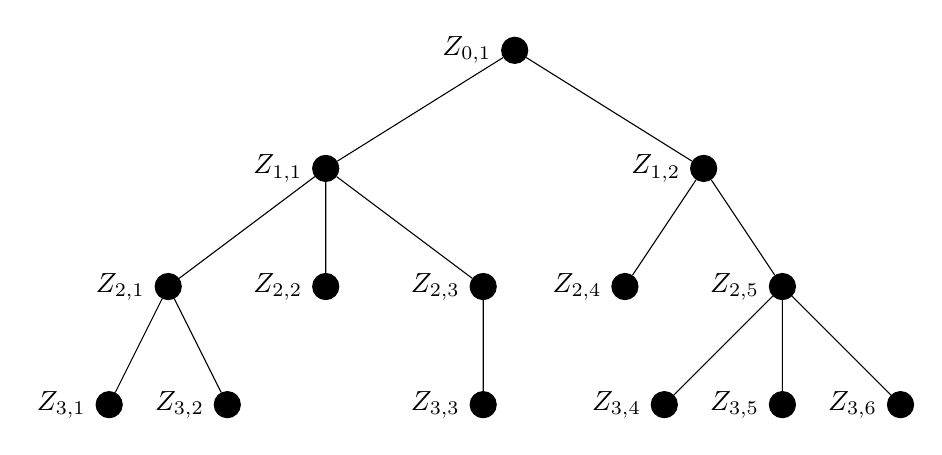
\begin{tikzpicture}[level distance=1.3cm,
        vertex/.style={minimum size=0.5pt,fill,draw,circle},
        level 1/.style={sibling distance=4.8cm, level distance=1.5cm},
        level 2/.style={sibling distance=2cm, level distance=1.5cm},
        level 3/.style={sibling distance=1.5cm, level distance=1.5cm},
        leaf/.style={label={[name=#1]left:$#1$}},
        ]
        \node[vertex, leaf = Z_{0,1}] {}
        child {node[vertex, leaf = Z_{1,1}] {}
            child {node[vertex, leaf = Z_{2,1}] {}
            child {node[vertex, leaf = Z_{3,1}] {}}
            child {node[vertex, leaf = Z_{3,2}] {}}
            }
            child {node[vertex, leaf = Z_{2,2}] {}}
            child {node[vertex, leaf = Z_{2,3}] {}
            child {node[vertex, leaf = Z_{3,3}] {}}
            }
        }
        child {node[vertex, leaf = Z_{1,2}] {}
            child {node[vertex, leaf = Z_{2,4}] {}}
            child {node[vertex, leaf = Z_{2,5}] {}
            child {node[vertex, leaf = Z_{3,4}] {}}
            child {node[vertex, leaf = Z_{3,5}] {}}
            child {node[vertex, leaf = Z_{3,6}] {}}
            }
        };
        \end{tikzpicture}
        \end{center}
    \item $ z $-transform for distribution of $ X_t $:
    \begin{align}
        \Pi_t(s)=\mathbb{E}\left[ s^X_t \right] = \sum_{j=0}^\infty s^j\mathbb{P}\left( X_t=j \right)  \quad L(s)=\mathbb{E}\left[ s^Z \right] =\sum_{j=0}^\infty s^j\mathbb{P}\left( Z=j \right) 
    \end{align}
    and 
    \begin{align}
        \Pi_t(s)=&\sum_{j=0}^\infty \mathbb{E}\left[ s^{X_t}|X_{t-1}=h \right] \mathbb{P}\left( X_{t-1}=j \right) \\
        =&\sum_{j=0}^\infty \left(L(s)\right)^{j}\mathbb{P}\left( X_{t-1}=j \right) \\
        =&\Pi_{t-1}\left(L(s)\right)\\
        (\Pi_1(s)=L(s))=&L^{(t)}(s) 
    \end{align}
    \item Mean and Variance:
    \begin{align}
        \text{Mean}:&\, \mu (t) = \Pi_t'(1)=\mu(0) ^t\\
        \text{Variance}:&\,var(t)=\Pi_t''(1)+\Pi_t'(1)-[\Pi_t'(1)]^2
    \end{align}
    \item Extinction Probability\index{Extinction Probability}
    \begin{align}
        \theta _t=&\mathbb{P}\left( X_t=0 \right)= \sum_{j=0}^\infty \theta ^j_{t-1}\mathbb{P}\left( Z=j \right) \\=
        &L(\theta _{t-1})
    \end{align}
    The eventual extinction is $ \theta ^*=L(\theta ^*) $, the fixed point of $ L(\, \cdot \, ) $.
    There is a phase transformation at $ \mu = 1 $
    \begin{align}
        \mathbb{P}\left( \theta ^*=1 \right) =\begin{cases}
            1,&\mu \leq 1\\
            \text{the first root of }L(\theta )=\theta ,& \mu >1
        \end{cases} 
    \end{align}
    
    Convergence order at phase transition point:
    \begin{align}
        \mathbb{P}\left( X_T>n \right) \sim \begin{cases}
            c_1\mu ^n,&\mu <1\\
            \dfrac{c_2}{n},&\mu =1
        \end{cases}  
    \end{align}
     
\end{itemize}


\subsection{Brownian Motion}
\index{Brownian Motion}\index{Wiener Process}\hypertarget{BrownianProcess}{}

Motivation: Brownian motion / Weiner Process $ W_t $\footnote{Symbol $ W_t $ for `Wiener', sometimes uses $ B_t $ for `Brown'.} is similar to a random walk model with $ p=q=1/2 $, but with initial state $ X_0=0 $, and `steps' defined as `a short enough time segmentation'.
\begin{align}
    W_{t=\frac{k}{N}}:= \dfrac{1}{\sqrt{N}} \sum_{i=1}^k \varpi _i,\quad \varpi _i\sim_{\mathrm{i.i.d.} } \mathrm{Unif}\{+1,-1\} 
\end{align}
and have $ N\to \infty $ as a Brownian Motion (Donsker Theorem\index{Donsker Theorem})

Rigorous definition of \textbf{Brownian / Wiener Process}: $ \{W_t:T\geq 0\} $ with $ 0<\sigma ^2<\infty $ is Brownian if
\begin{enumerate}[topsep=2pt,itemsep=2pt]
    \item Starts from $ 0 $: $ \mathbb{P}\left( W_0 \right) =1 $
    \item Independent increment: $ W_{t_1}-W_{s_1}\independent W_{t_2}-W_{s_2} $, $  \forall [t_1,s_1]\cap [t_2,s_2]=\emptyset $
    \item Zero mean Normal: $ W_t-W_s\sim N(0,\sigma ^2\vert t-s\vert) $
    \item continuity: $ \mathbb{P}\left( W_t\text{ continuous} \right) =1 $ 
\end{enumerate}

Properties:
\begin{itemize}[topsep=2pt,itemsep=0pt]
        \item Parameters
        \begin{align}
            \begin{cases}
                \text{Mean Function}:\mu (t)=0\\
                \text{Covariance}:\gamma (t,s)=\sigma ^2 \min\{s,t\} 
            \end{cases} 
        \end{align}
        \item m.s. indifferentiable
        \begin{align}
            \mathbb{E}\left[ \left(\dfrac{\partial^{} W_t}{\partial t^{}}\right)^2 \right]\to \infty  
        \end{align}
        which is the reason why the plots for Brownian Motion always looks rugged.
        \item Conditional distribution / Brownian Bridge $ B_t $:
        \begin{align}
            B_t := W_t|W_T=0 \sim N(0,\sigma ^2\dfrac{t(T-t)}{T})
        \end{align}
        \begin{itemize}[topsep=2pt,itemsep=0pt]
            \item Dependent increment: non-zero covariance
        \begin{align}
            \gamma_\mathrm{Bridge}  (t,s) = \sigma ^2\left(\min\{t,s\}-\dfrac{ts}{T}\right)
        \end{align}
            \item Cross definition between Wiener Process and Brownian Bridge:
            \begin{align}
                \begin{cases}
                    B_t:=W_t-\dfrac{t}{T}W_T\\
                    W_t:=B_t+t \sigma ^2 N(0,1) 
                \end{cases}
            \end{align}
            i.e. Brownian Bridge is independent of the terminal of its corresponding Wiener Process $ B_t\independent W_T $.
        \end{itemize}
\end{itemize}

\subsection{Poisson Process}\label{SubSubSectionPoissonProcess}
\index{Poisson Process}\hypertarget{PoissonProcess}{}

Motivation: The accumulate events happens at random, with `happening rate' of events as $ \lambda  $
\begin{align}
    N_{t=\frac{k}{N}}:= \sum_{i=1}^k \nu  _i,\quad \nu  _i\sim_{\mathrm{i.i.d.} } \mathrm{Bern}(\dfrac{\lambda }{n}) 
\end{align}

Rigorous Definition of \textbf{Poisson Process}: $ \{N_t:t\geq 0\} $ with rate $ \lambda >0 $ is Poisson if 
\begin{itemize}[topsep=2pt,itemsep=0pt]
    \item Counting Process $ N_t $: $ N_0=0 $, $ N_t\in\mathbb{N} $
    \item Independent Increment: $ N_{t_1}-N_{s_1}\independent N_{t_2}-N_{s_2} $, $ \forall [t_1,s_1\cap [t_2,s_2]=\emptyset $
    \item Poisson increment: $ N_t-N_s\sim P\left(\lambda (t-s)\right) $, $ t\geq s $\footnote{A proof \& another kind of definition concerning the intuition of `rate $ \lambda  $' is here: \url{https://v1ncent19.github.io//texts/Poisson/}.}
\end{itemize}

Properties:
\begin{itemize}[topsep=2pt,itemsep=0pt]
    \item Parameters
    \begin{align}
        \begin{cases}
            \text{Mean Function}:\mu (t)=\lambda t\\
            \text{Covariance}:\gamma (t,s)=\lambda \min\{s,t\} 
        \end{cases}
    \end{align}
    \item Arrival time: $ N_{t_n}=n $ means there are $ n $ events before (and including) $ t_n $, denoted $ \{t_1,t_2,\ldots,t_n\} $. PDF
    \begin{align}
        f_{T_1,T_2,\ldots,T_n}(t_1,t_2,\ldots,t_n)=\lambda ^ne^{-\lambda t_n}\mathbb{I}_{0<t_1<t_2<\ldots<t_n}
    \end{align}
    \item Inter-event time: PDF of time-between-events $ \{u_1,u_2,\ldots,u_n\}:=\{t_1,t_2-t_1,\ldots,t_n-t_{n-1}\} $
    \begin{align}
        f_{U_1,U_2,\ldots,U_n}(u_1,u_2,\ldots,u_n)=\prod_{i=1}^n \lambda e^{-\lambda u_i}\mathbb{I}_{u_i\geq 0}=\sim \otimes{i=1}^n\varepsilon_i (\lambda )
    \end{align}
    
    i.e. time-between-events satisfies exponential distribution
    \begin{align}
        U_i\sim_\mathrm{i.i.d.}  \varepsilon (\lambda ) 
    \end{align}

    \item Conditional distribution
    \begin{align}
        f_{T_1,T_2,\ldots,T_n|N_t=n}(t_1,t_2,\ldots,t_n)=\dfrac{n!}{t^n}\mathbb{I}_{0<t_1<t_2<\ldots<t_n}\sim \mathrm{Unif}\left(\mathbb{I}_{0<t_1<t_2<\ldots<t_n\leq t}\right) 
    \end{align}
    is the PDF of order statistics\footnote{See \autoref{EqaDistributionOfOrderStatistics}.} of i.i.d. $ \mathrm{Unif}(0,t)  $.
    \item Poisson Process and Martingale: 
    \begin{align}
        \tilde{N}_t:=N_t-\lambda t\sim\mathrm{Martingale}  
    \end{align}
    
\end{itemize}


\subsection{Birth-Death Process}
\index{Birth-Death Process}
Birth-death process looks like a one-end random-walk with `step' as poisson r.v.(i.e. exponential time-interval) The transition rate \& diagram are:
\begin{center}
    $
    Q=\begin{pNiceMatrix}[first-row,first-col]
        &0&1&2&3&\cdots\,\,\\
        0&-\lambda _0&\lambda _0&&&\\
        1&\mu _1&-\mu _1-\lambda _1&\lambda _1&&\\
        2&&\mu _2&-\mu _2-\lambda _2&\lambda _2&\\
        3&&&\mu _3&\ddots&\ddots\\
        \vdots&&&&\ddots&\ddots
        % \vdots&&&&&1\\
    \end{pNiceMatrix}\qquad \bm{\leftrightharpoons }\qquad
    $
    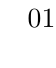
\begin{tikzpicture}[baseline={([yshift = -1ex]current bounding box.center)}]
    \GraphInit[vstyle=Dijkstra]
    \SetGraphUnit{2}
        \tikzset{VertexStyle/.style = {
            shape = rectangle,
            color = black,
            text = black,
            inner sep = 2pt,
            outer sep = 2pt,
            draw}}
        \Vertex[L=$ 0 $]{0}
        \EA[L=$1$](0){1}
        \EA[L=$2$](1){2}
        % \EA[L=$3$](2){3}
        \tikzset{VertexStyle/.style = {
            shape = circle,
            color = white,
            text = black,
            minimum size = 23pt,
            draw}}
        \EA[L=...,unit=1.9 ](2){3}

        \tikzset{EdgeStyle/.style = {->,bend left,thick}}
        \tikzset{LabelStyle/.style = {fill=white}}
        \Edge[label=$ \lambda _0 $](0)(1)
        \Edge[label=$ \lambda _1 $](1)(2)
        \Edge[label=$ \lambda _2 $](2)(3)
        % \Edge[label=$ \lambda _3 $](3)(4)

        \Edge[label=$ \mu _1 $](1)(0)
        \Edge[label=$ \mu _2 $](2)(1)
        \Edge[label=$ \mu _3 $](3)(2)
        % \Edge[label=$ \mu _4 $](4)(3)

    \end{tikzpicture}
    \end{center}

\begin{itemize}[topsep=2pt,itemsep=0pt]
    \item Kolmogorov forward: with a trivial notation that $ \lambda _{-1}=\mu _0=0 $, we have
    \begin{align}
         \dot{p}_i(t)=\lambda _{i-1}p_{i-1}(t)+\mu _{i+1}p_{i+1}(t)-(\lambda _i+\mu _i)p_i(t)
    \end{align}
    \item Stationary Distribution: $ \dot{\pi}^*=0 $ yields 
    \begin{align}
        (\lambda _i+\mu _i)\pi_i^*=\lambda _{i-1}\pi_{i-1}^*+\mu _{i+1}\pi^*_{i+1} 
    \end{align}
    Solution:
    \begin{align}
        \pi^*_i=\begin{cases}
            \dfrac{1}{Z}\dfrac{\lambda _0\lambda _1\ldots\lambda _{i-1}}{\mu _1\mu _2\ldots\mu _i},&i\neq 0\\
            \dfrac{1}{Z},&i=0
        \end{cases},\quad Z=1+\sum_{j=1}^\infty \dfrac{\lambda _0\lambda _1\ldots\lambda _{j-1}}{\mu _1\mu _2\ldots\mu _j}
    \end{align}
    
\end{itemize}








































\section{Applications}


\subsection{Innovation Sequence}
     
Motivation of Innovation Sequence (新息序列)\index{Innovation Sequence}: construction of linear MMSE $ L(X|Y_1,Y_2,\ldots,Y_n)=L(X|Y) $. Assume that $\mathbb{E}\left[ \vec{Y} \right] =0 $, the prediction is
\begin{align}
    L(X|\vec{Y})=\mathbb{E}\left[ X \right] + cov(X,\vec{Y})var(\vec{Y})^{-1}\vec{Y}
\end{align}
which causes the problem of computation complexity when dimension $ n $ is large. 

Innovation sequence fixed this problem by: instead of projecting on the whole linear combination $ \vec{Y} $ space of size $ (n+1) $, we project on space of each $ Y_i $ sequentially. i.e. define an \textbf{innovation sequence} 
\begin{align}
    \tilde{Y}_1=&Y_1-\mathbb{E}\left[ Y_1 \right] = Y_1 - \mathbb{E}\left[ Y_1 \right] \\
    \tilde{Y}_2=&Y_2-L(Y_2|Y_1) = Y_2-L(Y_2|\tilde{Y}_1)\\
    \tilde{Y}_3=&Y_3-L(Y_3|Y_2Y_1)= Y_3-L(Y_3|\tilde{Y}_2\tilde{Y}_1)\\
    \ldots&\\
    \tilde{Y}_n=&Y_n-L(Y_n|Y_{n-1}\ldots Y_2Y_1)=Y_n-L(Y_n|\tilde{Y}_{n-1}\ldots \tilde{Y}_2\tilde{Y}_1)
\end{align}
where `innovation' means each $ \tilde{Y}_i $ contains the `new information without correlation with previous sequence': $ \mathbb{E}\left[ \tilde{Y_i}\tilde{Y}_j \right]=0\,\forall i\neq j  $. Computation of innovation sequence:
\begin{align}
     \tilde{Y}_k=&Y_k-L(Y_k|\tilde{Y}_{k-1}\ldots \tilde{Y}_1)=Y_k-\mathbb{E}\left[ Y_k \right] -\sum_{j=1}^{k-1}\dfrac{cov(Y_k,\tilde{Y}_{j})}{var(\tilde{Y}_{j})}\tilde{Y}_j,\quad k=1,2,\ldots,n
\end{align}
with a trivial notation that $ Y_{0}=1 $

In this way a linear MMSE $ L(X|\vec{Y}) $ could be written as
\begin{align}
    L(X|\vec{Y})=L(X|\vec{\tilde{Y}})= \mathbb{E}\left[ X \right] +\sum_{i=1}^n \dfrac{cov(X,\tilde{Y}_i)}{var(\tilde{Y}_i)}\tilde{Y}_i=\mathbb{E}\left[ X \right] +\sum_{i=1}^n L\left(X-\mathbb{E}\left[ X \right] |\tilde{Y}_i\right)
\end{align}


I think the idea here is similar to Gram-Schmidt orthogonalization (\autoref{SubSubSectionQRDecomposition}), in which we also construct new components by eliminating projection on previous parts. As a result we have a set of orthogonal elements (here orthogonal means $ \mathbb{E}\left[ \tilde{Y}_i\tilde{Y}_j \right]=0  $ and in Gram-Schmidt means $ q_i'q_j = 0 $, $ i\neq j $). And the result is a `change of basis' of space.




\subsection{Markov Decision Processes}
\index{MDPs (Markov Decision Processes)}\index{Episode}\index{Policy}
In decision process/episode, say $ \{(s_t,a_t)\}_{t=0}^T $, we need to determine a \textbf{policy} $ \pi_t $ to take \textbf{action}  $ a_t $ given \textbf{state}  $ s_t $ as
\begin{align}
    a_t\sim \pi_t(\, \cdot \,| s_t) \text{ or simply }a_t=\pi_t(s_t)
\end{align}
then (conditional) \textbf{transition}  probability is a model pre-assumed, say
\begin{align}
    s_{t+1}\sim p_t\left(\, \cdot \, |s_t,a_t\right) 
\end{align}


\begin{point}
    Optimization Target
\end{point}

The optimization target (in each step) is \textbf{reward function} 
\begin{align}
    r_t(s_t,s_{t+1}|a_t)
\end{align}

The `cumulative reward' from step $ t $ is denoted $ \mathcal{V}_{t\leadsto T} $\footnote{In this subsection I usually use the superscript $ \cdot ^{\pi_{t:T}} $ to specify the optimize target.} 
\begin{align}\label{EqaVLearningIteration}
    \mathcal{V}_{t\leadsto T}^{\pi_{t:T}}(s_t)=\mathbb{E}_{s_{t+1}\sim p\left(\, \cdot \, |s_t,a_t=\pi(s_t)\right)}\left[ r_t\left(s_t,s_{t+1}|a_t=\pi_t(s_t)\right)+\gamma \mathcal{V}_{(t+1)\leadsto T}^{\pi_{(t+1):T}} (s_{t+1})\big|s_t\right]
\end{align}
where \textbf{discount factor} $ \gamma<1  $\index{Discount Factor} is induced to focus on recent rewards. By expanding all iteration terms we have
\begin{align}
    \mathcal{V}_{t\leadsto T}^{\pi_{t:T}}(s_t)=&\mathbb{E}_{s_{(t+1):(T+1)}}\left[ \sum_{\tau = t}^T\gamma ^{\tau-t}r_\tau\left(s_\tau,s_{\tau+1}|a_\tau=\pi_\tau(s_\tau)\right)\big|s_t \right]
\end{align}
and the final optimize goal is maximize total reward $ \mathcal{V} $
\begin{align}\label{EqaVLearningTarget}
    \pi_{0:T}^*=&\mathop{\arg\max}\limits_{\pi_{0:T}}\,\mathbb{E}_{s_0\sim p_0(\, \cdot \, )}\left[ \mathcal{V}_{0\leadsto T}^{\pi_{0:T}}(s_0) \right]  \\
    =&\mathop{\arg\max}\limits_{\pi_{0:T}}\,\mathbb{E}_{s_{0:(T+1)}}\left[ \sum_{\tau = 0}^T\gamma ^{\tau}r_\tau\left(s_\tau,s_{\tau+1}|a_\tau=\pi_\tau(s_\tau)\right) \right]
\end{align}



Comments:
\begin{itemize}[topsep=2pt,itemsep=0pt]
    \item The joint distribution of $ s_{t+1,T+1} $ has a complicated dependence on $ p_\tau(\, \cdot \, |s_\tau,a_\tau) $, making the optimization hard to solve directly.
    \item Actually when making decision we should consider a complete process, i.e. $ T\to \infty $, but note that with $ \gamma <1 $, reward at far future is dispensable if rewards are upper-bounded $ r_\tau(s_\tau,s_{\tau+1}|a_\tau)\leq \tilde{r} $, then
    \begin{align}
        \sum_{\tau = T }^\infty\gamma ^{\tau}r_\tau\left(s_\tau,s_{\tau+1}|a_\tau=\pi_\tau(s_\tau)\right) \leq \tilde{r}\dfrac{\gamma ^T}{1-\gamma }
    \end{align}
    which can be bounded below $\varepsilon  \tilde{r} $ for a large enough \textbf{Effective Length}  $ T_\varepsilon  $
    \begin{align}
        \tilde{r}\dfrac{\gamma ^T}{1-\gamma }<\tilde{r}\varepsilon \Rightarrow T_\varepsilon \approx \dfrac{\log[(1-\gamma )\varepsilon ]}{\log \gamma }\sim \mathcal{O}\left( \dfrac{1}{1-\gamma }\log\dfrac{1}{\varepsilon (1-\gamma )} \right)\sim \mathcal{O}(\dfrac{1}{1-\gamma })
    \end{align}
\end{itemize}

\begin{point}
    Algorithm
\end{point}

Solving all $ \pi_{0:T} $ jointly in \autoref{EqaVLearningTarget} is complex. It would be wiser to use the iteration form \autoref{EqaVLearningIteration} and \textit{separate decision making} $ a_t $ \textit{and processing} $ p(\, \cdot \, |s_t,a_t) $. With expected rewards denoted
\begin{align}
    R_t(s_t,a_t)= \mathbb{E}_{s_{t+1}\sim p\left(\, \cdot \, |s_t,a_t\right)}\left[ r_t(s_t,s_{t+1}|a_t)\big| s_t,a_t \right]
\end{align}
total reward $ \mathcal{V}_{t\leadsto T} $ could be written as\footnote{Here the ugly symbol means, e.g.
\begin{align*}
     \mathcal{V}_{\text{describes the process from when to when} }^{\text{is influenced by which policies }\pi_{\cdot }}(\text{as a function of which state})
\end{align*}
}
\begin{align}
    \mathcal{V}_{t\leadsto T}^{\pi_{t:T}}(s_t)=&\mathbb{E}_{s_{t+1}\sim p\left(\, \cdot \, |s_t,a_t\sim\pi(s_t)\right)}\left[ r_t\left(s_t,s_{t+1}|a_t\sim \pi_t(s_t)\right)+\gamma \mathcal{V}_{(t+1)\leadsto T}^{\pi_{(t+1):T}} (s_{t+1})\Big|s_t\right] \\
    =&{\color{red}\mathbb{E}_{a_t\sim \pi(\, \cdot \, |s_t)}\left[{\color{blue}R_{t}\left(s_t,a_t\right)+  \gamma\mathbb{E}_{s_{t+1}\sim p\left(\, \cdot \, |s_t,a_t\right)}\left[{\color{black}  \mathcal{V}_{(t+1)\leadsto T}^{\pi_{(t+1):T}} (s_{t+1})} \Big| s_t,a_t \right]}  \big|s_t\right]}
\end{align}
with the {red} part as \textbf{State-Value Function}\index{V-Value@$ V $-Value (State-Value Function)}\index{State-Value Function}, or {\color{red}$ V $-value}; the {blue} part as \textbf{Action-Value Function}\index{Action-Value Function}, or {\color{blue}$ Q $-value}
\begin{align}
    {\color{red}V_{t\leadsto T}^{\pi_{t:T}}(s_t)}=&\mathbb{E}_{a_t\sim \pi(\, \cdot \, |s_t)}\left[ Q_{t\leadsto T}^{\pi_{(t+1):T}}(s_t,a_t)  \big|s_t\right]\\
    {\color{blue}Q_{t\leadsto T}^{\pi_{(t+1):T}}(s_t,a_t)}=&R_t\left(s_t,a_t\right)+\gamma \mathbb{E}_{s_{t+1}\sim p\left(\, \cdot \, |s_t,a_t\right)}\left[V_{(t+1)\leadsto T}^{\pi_{(t+1):T}} (s_{t+1})\Big| s_t,a_t\right]
\end{align}

Comments:
\begin{itemize}[topsep=2pt,itemsep=0pt]
    \item The decision process $(s_0,a_0)\leadsto (s_1,a_1)\leadsto\ldots\leadsto (s_T,a_T) $
    is Markovian in $ t=0\leadsto T $ sense, while the reward propagation $ V_{T\leadsto T}\leadsto Q_{(T-1)\leadsto T}\leadsto V_{(T-1)\leadsto T}\leadsto \ldots\leadsto Q_{0\leadsto T}\leadsto V_{0\leadsto T} $ is `Markovian' in $t= T\leadsto 0 $ sense. i.e. solution to optimal $ \pi^* $ obtained by maximizing total reward should go backward.
    \item Duality of optimal $ \{V_{t\leadsto T}^{\pi_{t:T}}\}_{t=0}^T $ ($ V $-learning) and optimal $ \{Q_{t\leadsto T}^{\pi_{t:T}}\}_{t=0}^{T} $ ($ Q $-learning): With $ R_{t}(s_t,a_t) $ actually a given function (for given model $ p(s_{\tau+1}|s_\tau,a_\tau) $),
    \begin{align}
        \begin{cases}
            V_{t\leadsto T}^{\pi_{t:T}}(s_t)={\mathbb{E}_{\color{brown}a_t\sim \pi(\, \cdot \, |s_t)}\left[{R_{t}\left(s_t,a_t\right)+  \gamma\mathbb{E}_{s_{t+1}\sim p\left(\, \cdot \, |s_t,a_t\right)}\left[{\color{black}  V_{(t+1)\leadsto T}^{\pi_{(t+1):T}} (s_{t+1})} \Big| s_t,a_t \right]}  \big|s_t\right]}\\
            Q_{t\leadsto T}^{\pi_{(t+1):T}}(s_t,a_t)=R_t(s_t,a_t)+\gamma \mathbb{E}_{s_{t+1}\sim p\left(\, \cdot \, |s_t,a_t\right)}\left[ \mathbb{E}_{\color{brown}a_{t+1}\sim \pi(\, \cdot \, |s_{t+1})}\left[ Q_{(t+1)\leadsto T}^{\pi_{(t+2):T}}(s_{t+1},a_{t+1})  \big|s_{t+1}\right]  \Big| s_{t+1},a_{t+1}\right]
        \end{cases} 
    \end{align}
    are equivalent, with the same optimization core $ \mathbb{E}_{a_\tau\sim\pi(\, \cdot \, |s_\tau)}\left[ \, \cdot \,  |s_\tau \right]  $. 
    \item[$ \Delta  $] Value function iteration for optimal policy $ \pi^* $:
    \begin{align}
        \pi^*_t(s)=\mathop{\arg\max}\limits_{a} Q_t^*(s,a) ,\quad t=T,T-1,\ldots,0
    \end{align}
    
\end{itemize}
\begin{algorithm}{Value Iteration}
        \begin{enumerate}[topsep=2pt,itemsep=2pt]
            \item $ V^*_{T+1}\equiv 0 $
            \item \textit{for} $ t=T,T-1,\ldots,1 $
            \begin{enumerate}[topsep=2pt,itemsep=2pt]
                \item $ Q $-expectation step:
                \begin{align}
                  Q^*_t(s,a)=R_t(s,a)+\gamma \mathbb{E}_{\tilde{s}\sim p(\, \cdot \, |s,a)}\left[ V^*_{t+1}(\tilde{s}) \big|s,a\right]    
                \end{align}
                \item $ V $-Optimal step:
                \begin{align}
                     \begin{cases}\label{EqaValueIterationProcess}
                        \pi^*_t(s)=&\mathop{\arg\max}\limits_{a}Q_t^*(s,a)\\
                        V^*_t(s)= & \mathop{\max}\limits_{a} Q^*_t(s,a)=Q^*_{t}(s,\pi^*_t(s)) 
                     \end{cases}
                \end{align}
            \end{enumerate}
            i.e. a $ (Q_t,V_t) $ `backward propagation'.
        \end{enumerate}
    \end{algorithm}

\begin{point}
    $ Q $-Learning\index{Q-Learning@$ Q $-Learning}
\end{point}

Motivation: for some more complex cases, e.g.
\begin{itemize}[topsep=2pt,itemsep=0pt]
    \item The functional form of reward $ r_t(s_t,s_{t+1}|a_t) $ or $ R_{t}(s_t,a_t) $ is unknown
    \item The transition probability $ s_{t+1}\sim p(\, \cdot \, |s_t,a_t) $ is unknown
    \item The phase space is too large to compute point wise
\end{itemize}
Note that the above optimize process \autoref{EqaValueIterationProcess} is an optimization w.r.t. $ Q_t(\, \cdot \, ,\, \cdot \, ) $, we can first learn the functional form of $ Q(\, \cdot \, ,\, \cdot \, ) $ (or its function approximation), and thus get the policy $ \pi^* $. The $ Q $-learning process can have the following form:
\begin{align}
    \hat{Q}^{(\tau+1)}(s_{t},a_{t})\leftarrow \overbrace {\hat{Q}^{(\tau)}(s_{t},a_{t})}^{\text{current value}}+\alpha \cdot \overbrace{\bigg(\underbrace {R_t(s_t,a_t)+\gamma \cdot \underbrace {\max _{a}\hat{Q}^{(\tau)}(s_{t+1},a)} _{\text{estimate of optimal future value}}} _{\text{new value (temporal difference target)}}-\underbrace {\hat{Q}^{(\tau)}(s_{t},a_{t})} _{\text{current value}}\bigg )} ^{\text{temporal difference}}
\end{align}
with some known \textit{final/terminal} state $ \{s_\mathrm{final} \} $, where $ Q(s_\mathrm{final},a )\equiv 0,\,\forall a $


\begin{algorithm}{$ Q $-Learning}
\begin{enumerate}[topsep=2pt,itemsep=2pt]
    \item Initialize a tentative $ Q^{(0)}_{t}(\, \cdot \, ,\, \cdot \, ) $, say $ Q\equiv 0 $
    \item \textit{for} $ \tau=0,1,2,\ldots $ \textit{until} $ Q(\, \cdot \, ,\, \cdot \, ) $ converge:
    \begin{enumerate}[topsep=2pt,itemsep=2pt]
        \item Initialize some $ s_1 $
        \item \textit{for} $ t=1,2,\ldots $ \textit{until} $ s_{t}\in\{s_\mathrm{final} \} $: optimize the function form (approximation) $ Q(\, \cdot \, ,\, \cdot \, ) $
        \begin{align}
            \hat{Q}^{(\tau+1)}(s_t,a_t)\leftarrow& \hat{Q}^{(\tau)}(s_t,a_t)+\alpha \left(R_t(s_t,a_t)+\gamma \mathop{\max}\limits_{a}\hat{Q}^{(\tau)}_{t+1}(s_{t+1},a)-\hat{Q}^{(\tau)}_t(s_t,a_t) \right)\\
            s_{t+1}\leftarrow& p_t(s_t,a_t)
        \end{align}
    \end{enumerate}
\end{enumerate}
\end{algorithm}
    



% $ \lim_{u\to\infty}C_X(u)=0 \Rightarrow \forall \varepsilon >0,\,\exists u_\varepsilon $ s.t. $ C_X(u_\varepsilon )<\varepsilon  $, then for $ T $ large enough
% \begin{align}
%     \dfrac{2}{T}\int_{0}^T(1-\dfrac{\tau}{T})C_X(\tau)\,\mathrm{d}\tau =&\dfrac{2}{T}\left[\int_{0}^{u_\varepsilon }(1-\dfrac{\tau}{T})C_X(\tau)\,\mathrm{d}\tau + \int_{u_\varepsilon }^T(1-\dfrac{\tau}{T})C_X(\tau)\,\mathrm{d}\tau\right]\\
%     \leq&\dfrac{2}{T} \int_{0}^{u_\varepsilon }C_X(0)\,\mathrm{d}\tau +\dfrac{2}{T} \int_{0 }^T (1-\dfrac{\tau}{T})\varepsilon \,\mathrm{d}\tau  \\
%     =&\dfrac{2u_\varepsilon C_X(0)}{T}+\varepsilon \leq (2C_X(0)+1)\varepsilon 
% \end{align}



% General definition of Ergodicity: for any given $ \{t_1,t_2,\ldots,t_m\} $
% \begin{align}
%     \lim_{T\to\infty}\int_{0}^\infty f(X_{t_1+\tau},X_{t_2+\tau},\ldots,X_{t_m+\tau})\,\mathrm{d}\tau = \mathbb{E}\left[ f(X_{t_1},X_{t_2},\ldots,X_{t_m}) \right]  
% \end{align}

% e.g. stationary Gaussian with $ \mathrm{Cross}_X(\tau)\to 0   $ is ergodic in m.s. and a.s. sense.


\subsection{Karhunen-Loève Expansion}

Karhunen-Loève Expansion (KL Expansion)\index{KL Expansion (Karhunen-Loève Expansion)}\index{PCA (Principal Component Analysis)} is a coutinuous version of PCA \autoref{EqaCurseOfDimensionality}. The idea is a decomposition 
\begin{align}
    X(t)=\sum_{i}X_i\phi _i(t) 
\end{align}
i.e. we add an extra step in mapping
\begin{align}
    X(\, \cdot \, ):\, \Omega\mapsto \{X_i\}\mapsto \mathcal{T}\times \mathbb{R}  
\end{align}
a special set of $ \{X_i,\phi_i\} $ is given by KL expansion.

\begin{point}
    Derivations
\end{point}

First note that $ R(s,t):=\mathbb{E}\left[ X(s)X(t) \right] $ is a Kernel (see \autoref{EqaKernelFunction}), with positive semi-definition and symmetry. Then by Mercer's Theorem, it has eigen-function decomposition
\begin{align}
    R(s,t) =\sum_{i} \lambda _i\phi _i(s)\phi _i(t) \Leftrightarrow \langle R(s,\, \cdot \, ),\phi_i\rangle = \lambda _i\phi_i(s)
\end{align}
where eigen functions are orthonormal
\begin{align}
    \langle \phi _i, \phi _j \rangle := \int_\tau \phi _i(\tau)\phi _j(\tau)\,\mathrm{d}\tau = \delta _{ij}
\end{align}

using $ \{\phi _i\} $ as function basis, KL coefficients are r.v. 
\begin{align}
    X_i=\langle X_t, \phi _i\rangle  
\end{align}
with
\begin{align}
    \mathbb{E}\left[ X_iX_j \right] = \langle \phi_i | X_t\rangle \langle X_t| \phi_j\rangle =  \langle \phi_i | R(s,t) | \phi_j\rangle = \delta _{ij}\lambda _i
\end{align}

\begin{point}
Other Concepts
\end{point}
\begin{itemize}[topsep=2pt,itemsep=0pt]
    \item Total energy:
    \begin{align}
        E=\mathbb{E}\left[ \left\langle X_t,X_t \right\rangle \right]=\sum_i\lambda _i
    \end{align}
    \item Rank: $ \mathrm{rank}\left(\{\mathbb{E}\left[ X_iX_j \right] \}\right) = \#(\lambda _i\neq 0) $ is also the rank of the process.
    
\end{itemize}

    














\subsection{Kalman Filter}
\begin{point}
    Model
\end{point}

    \textbf{Kalman Filter}\index{Kalman Filter} is an auto-regressive / iterative filter for estimating the \textbf{state} $ x_t $ from \textbf{observable}\footnote{Here I prefer the name as in Quantum mechanics `Observable'.} $ z_t $. The model structure, as in \autoref{FigKalmanStructure}, is a Hidden Markov Model (HMM)\index{HMM (Hidden Markov Model)} with linear operator.
    \begin{align}
        \text{State: }&x_{k}=F_{k}x_{k-1}+w_{k} \\
        \text{Observable: }&z_{k}=H_kx_k+v_k
    \end{align}  
    where $ w_k,\,v_k $ is noise / random error, usually with (multivariate) Normal distribution
    \begin{align}
        w_k\sim N(0,Q_k),\qquad v_k\sim N(0,R_k) 
    \end{align}
    the initial state denoted
    \begin{align}
        x_0\sim N(\hat{x}_{0|0}, P _{0|0}) 
    \end{align}

\begin{figure}[H]
    \centering
    

\tikzset{every picture/.style={line width=0.75pt}} %set default line width to 0.75pt        

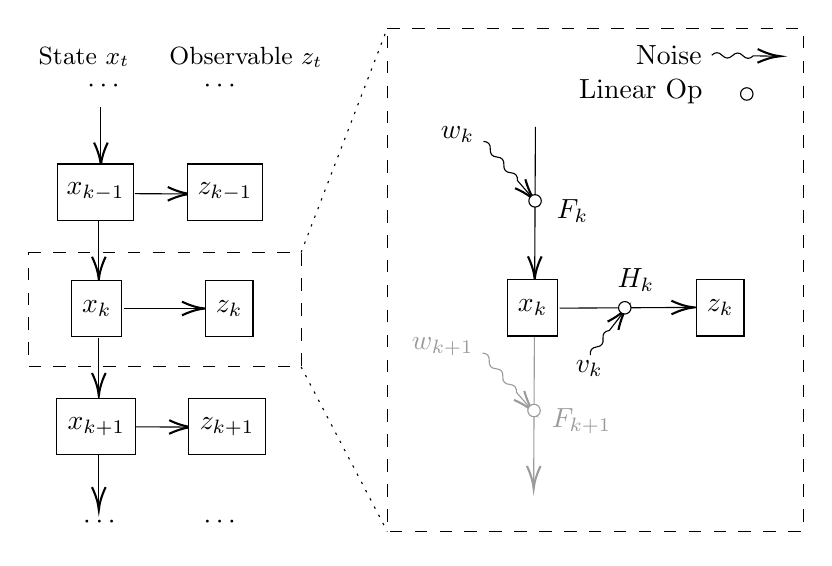
\begin{tikzpicture}[x=0.75pt,y=0.75pt,yscale=-1,xscale=1]
%uncomment if require: \path (0,300); %set diagram left start at 0, and has height of 300

%Straight Lines [id:da8051072890440967] 
\draw [color={rgb, 255:red, 0; green, 0; blue, 0 }  ,draw opacity=1 ][fill={rgb, 255:red, 255; green, 255; blue, 255 }  ,fill opacity=1 ]   (251.33,83.49) .. controls (253.68,83.66) and (254.78,84.92) .. (254.61,87.27) .. controls (254.44,89.62) and (255.53,90.88) .. (257.88,91.05) .. controls (260.23,91.22) and (261.33,92.48) .. (261.16,94.83) .. controls (260.99,97.18) and (262.08,98.43) .. (264.43,98.6) .. controls (266.78,98.77) and (267.88,100.03) .. (267.71,102.38) -- (269.64,104.61) -- (274.88,110.66) ;
\draw [shift={(276.19,112.17)}, rotate = 229.09] [color={rgb, 255:red, 0; green, 0; blue, 0 }  ,draw opacity=1 ][line width=0.75]    (10.93,-3.29) .. controls (6.95,-1.4) and (3.31,-0.3) .. (0,0) .. controls (3.31,0.3) and (6.95,1.4) .. (10.93,3.29)   ;
%Straight Lines [id:da8443065915101042] 
\draw    (66.01,122.03) -- (66.01,148.03) ;
\draw [shift={(66.01,150.03)}, rotate = 270] [color={rgb, 255:red, 0; green, 0; blue, 0 }  ][line width=0.75]    (10.93,-3.29) .. controls (6.95,-1.4) and (3.31,-0.3) .. (0,0) .. controls (3.31,0.3) and (6.95,1.4) .. (10.93,3.29)   ;
%Straight Lines [id:da6875878363586321] 
\draw    (66.01,178.03) -- (66.01,204.03) ;
\draw [shift={(66.01,206.03)}, rotate = 270] [color={rgb, 255:red, 0; green, 0; blue, 0 }  ][line width=0.75]    (10.93,-3.29) .. controls (6.95,-1.4) and (3.31,-0.3) .. (0,0) .. controls (3.31,0.3) and (6.95,1.4) .. (10.93,3.29)   ;
%Straight Lines [id:da05843745637022657] 
\draw    (78.01,164.03) -- (115.01,164.03) ;
\draw [shift={(117.01,164.03)}, rotate = 180] [color={rgb, 255:red, 0; green, 0; blue, 0 }  ][line width=0.75]    (10.93,-3.29) .. controls (6.95,-1.4) and (3.31,-0.3) .. (0,0) .. controls (3.31,0.3) and (6.95,1.4) .. (10.93,3.29)   ;
%Straight Lines [id:da11088548439510282] 
\draw    (67.01,67.03) -- (67.01,93.03) ;
\draw [shift={(67.01,95.03)}, rotate = 270] [color={rgb, 255:red, 0; green, 0; blue, 0 }  ][line width=0.75]    (10.93,-3.29) .. controls (6.95,-1.4) and (3.31,-0.3) .. (0,0) .. controls (3.31,0.3) and (6.95,1.4) .. (10.93,3.29)   ;
%Straight Lines [id:da19051414013865076] 
\draw    (66.01,233.03) -- (66.01,259.03) ;
\draw [shift={(66.01,261.03)}, rotate = 270] [color={rgb, 255:red, 0; green, 0; blue, 0 }  ][line width=0.75]    (10.93,-3.29) .. controls (6.95,-1.4) and (3.31,-0.3) .. (0,0) .. controls (3.31,0.3) and (6.95,1.4) .. (10.93,3.29)   ;
%Straight Lines [id:da7993986672570081] 
\draw    (83.34,108.7) -- (108.16,108.82) ;
\draw [shift={(110.16,108.83)}, rotate = 180.29] [color={rgb, 255:red, 0; green, 0; blue, 0 }  ][line width=0.75]    (10.93,-3.29) .. controls (6.95,-1.4) and (3.31,-0.3) .. (0,0) .. controls (3.31,0.3) and (6.95,1.4) .. (10.93,3.29)   ;
%Straight Lines [id:da6382436414377908] 
\draw    (84.01,221.03) -- (108.83,221.16) ;
\draw [shift={(110.83,221.17)}, rotate = 180.29] [color={rgb, 255:red, 0; green, 0; blue, 0 }  ][line width=0.75]    (10.93,-3.29) .. controls (6.95,-1.4) and (3.31,-0.3) .. (0,0) .. controls (3.31,0.3) and (6.95,1.4) .. (10.93,3.29)   ;
%Rounded Rect [id:dp614251386292366] 
\draw  [dash pattern={on 4.5pt off 4.5pt}] (32,137) .. controls (32,137) and (32,137) .. (32,137) -- (163.49,137) .. controls (163.49,137) and (163.49,137) .. (163.49,137) -- (163.49,192.17) .. controls (163.49,192.17) and (163.49,192.17) .. (163.49,192.17) -- (32,192.17) .. controls (32,192.17) and (32,192.17) .. (32,192.17) -- cycle ;
%Straight Lines [id:da642038681386998] 
\draw [color={rgb, 255:red, 0; green, 0; blue, 0 }  ,draw opacity=1 ][fill={rgb, 255:red, 255; green, 255; blue, 255 }  ,fill opacity=1 ]   (276.37,76.48) -- (276.02,147.86) ;
\draw [shift={(276.01,149.86)}, rotate = 270.28] [color={rgb, 255:red, 0; green, 0; blue, 0 }  ,draw opacity=1 ][line width=0.75]    (10.93,-3.29) .. controls (6.95,-1.4) and (3.31,-0.3) .. (0,0) .. controls (3.31,0.3) and (6.95,1.4) .. (10.93,3.29)   ;
%Straight Lines [id:da3676361709618625] 
\draw    (288.01,163.86) -- (350.83,163.5) ;
\draw [shift={(352.83,163.49)}, rotate = 179.67] [color={rgb, 255:red, 0; green, 0; blue, 0 }  ][line width=0.75]    (10.93,-3.29) .. controls (6.95,-1.4) and (3.31,-0.3) .. (0,0) .. controls (3.31,0.3) and (6.95,1.4) .. (10.93,3.29)   ;
%Straight Lines [id:da8799353629961175] 
\draw    (302.83,186.49) .. controls (302.53,184.15) and (303.55,182.83) .. (305.89,182.53) .. controls (308.23,182.23) and (309.25,180.91) .. (308.94,178.57) .. controls (308.63,176.23) and (309.65,174.91) .. (311.99,174.61) -- (314.32,171.6) -- (319.2,165.26) ;
\draw [shift={(320.42,163.68)}, rotate = 127.63] [color={rgb, 255:red, 0; green, 0; blue, 0 }  ][line width=0.75]    (10.93,-3.29) .. controls (6.95,-1.4) and (3.31,-0.3) .. (0,0) .. controls (3.31,0.3) and (6.95,1.4) .. (10.93,3.29)   ;
%Straight Lines [id:da3845121992781433] 
\draw [color={rgb, 255:red, 155; green, 155; blue, 155 }  ,draw opacity=1 ]   (275.87,177.48) -- (275.52,248.86) ;
\draw [shift={(275.51,250.86)}, rotate = 270.28] [color={rgb, 255:red, 155; green, 155; blue, 155 }  ,draw opacity=1 ][line width=0.75]    (10.93,-3.29) .. controls (6.95,-1.4) and (3.31,-0.3) .. (0,0) .. controls (3.31,0.3) and (6.95,1.4) .. (10.93,3.29)   ;
%Straight Lines [id:da9798416569763584] 
\draw [color={rgb, 255:red, 155; green, 155; blue, 155 }  ,draw opacity=1 ]   (250.83,185.49) .. controls (253.18,185.66) and (254.28,186.92) .. (254.11,189.27) .. controls (253.94,191.62) and (255.03,192.88) .. (257.38,193.05) .. controls (259.73,193.22) and (260.83,194.48) .. (260.66,196.83) .. controls (260.49,199.18) and (261.58,200.43) .. (263.93,200.6) .. controls (266.28,200.77) and (267.38,202.03) .. (267.21,204.38) -- (269.14,206.61) -- (274.38,212.66) ;
\draw [shift={(275.69,214.17)}, rotate = 229.09] [color={rgb, 255:red, 155; green, 155; blue, 155 }  ,draw opacity=1 ][line width=0.75]    (10.93,-3.29) .. controls (6.95,-1.4) and (3.31,-0.3) .. (0,0) .. controls (3.31,0.3) and (6.95,1.4) .. (10.93,3.29)   ;
%Rounded Rect [id:dp9419817408683995] 
\draw  [dash pattern={on 4.5pt off 4.5pt}] (205,28.99) .. controls (205,28.99) and (205,28.99) .. (205,28.99) -- (405.33,28.99) .. controls (405.33,28.99) and (405.33,28.99) .. (405.33,28.99) -- (405.33,271.49) .. controls (405.33,271.49) and (405.33,271.49) .. (405.33,271.49) -- (205,271.49) .. controls (205,271.49) and (205,271.49) .. (205,271.49) -- cycle ;
%Straight Lines [id:da916303967111838] 
\draw  [dash pattern={on 0.84pt off 2.51pt}]  (163.49,137) -- (205,28.99) ;
%Straight Lines [id:da8876073772934547] 
\draw  [dash pattern={on 0.84pt off 2.51pt}]  (163.49,192.17) -- (205,271.49) ;
%Shape: Circle [id:dp27142797833084686] 
\draw  [color={rgb, 255:red, 0; green, 0; blue, 0 }  ,draw opacity=1 ][fill={rgb, 255:red, 255; green, 255; blue, 255 }  ,fill opacity=1 ] (273.19,112.17) .. controls (273.19,110.51) and (274.53,109.17) .. (276.19,109.17) .. controls (277.85,109.17) and (279.19,110.51) .. (279.19,112.17) .. controls (279.19,113.83) and (277.85,115.17) .. (276.19,115.17) .. controls (274.53,115.17) and (273.19,113.83) .. (273.19,112.17) -- cycle ;
%Shape: Circle [id:dp746836452749982] 
\draw  [fill={rgb, 255:red, 255; green, 255; blue, 255 }  ,fill opacity=1 ] (316.42,163.68) .. controls (316.42,162.02) and (317.76,160.68) .. (319.42,160.68) .. controls (321.08,160.68) and (322.42,162.02) .. (322.42,163.68) .. controls (322.42,165.33) and (321.08,166.68) .. (319.42,166.68) .. controls (317.76,166.68) and (316.42,165.33) .. (316.42,163.68) -- cycle ;
%Shape: Circle [id:dp7897054395526044] 
\draw  [color={rgb, 255:red, 155; green, 155; blue, 155 }  ,draw opacity=1 ][fill={rgb, 255:red, 255; green, 255; blue, 255 }  ,fill opacity=1 ] (272.69,213.17) .. controls (272.69,211.51) and (274.03,210.17) .. (275.69,210.17) .. controls (277.35,210.17) and (278.69,211.51) .. (278.69,213.17) .. controls (278.69,214.83) and (277.35,216.17) .. (275.69,216.17) .. controls (274.03,216.17) and (272.69,214.83) .. (272.69,213.17) -- cycle ;
%Straight Lines [id:da11141445571255759] 
\draw    (361.33,41.99) .. controls (363.02,40.35) and (364.69,40.38) .. (366.33,42.07) .. controls (367.98,43.76) and (369.64,43.78) .. (371.33,42.14) .. controls (373.02,40.5) and (374.69,40.53) .. (376.33,42.22) .. controls (377.98,43.91) and (379.64,43.93) .. (381.33,42.29) -- (384.33,42.34) -- (392.33,42.46) ;
\draw [shift={(394.33,42.49)}, rotate = 180.87] [color={rgb, 255:red, 0; green, 0; blue, 0 }  ][line width=0.75]    (10.93,-3.29) .. controls (6.95,-1.4) and (3.31,-0.3) .. (0,0) .. controls (3.31,0.3) and (6.95,1.4) .. (10.93,3.29)   ;
%Shape: Circle [id:dp11478084942637645] 
\draw  [fill={rgb, 255:red, 255; green, 255; blue, 255 }  ,fill opacity=1 ] (375.19,60.67) .. controls (375.19,59.01) and (376.53,57.67) .. (378.19,57.67) .. controls (379.85,57.67) and (381.19,59.01) .. (381.19,60.67) .. controls (381.19,62.33) and (379.85,63.67) .. (378.19,63.67) .. controls (376.53,63.67) and (375.19,62.33) .. (375.19,60.67) -- cycle ;

% Text Node
\draw  [fill={rgb, 255:red, 255; green, 255; blue, 255 }  ,fill opacity=1 ]  (45.93,94.42) -- (82.93,94.42) -- (82.93,121.42) -- (45.93,121.42) -- cycle  ;
\draw (64.43,107.92) node    {$x_{k-1}$};
% Text Node
\draw  [fill={rgb, 255:red, 255; green, 255; blue, 255 }  ,fill opacity=1 ]  (53.04,150.42) -- (77.04,150.42) -- (77.04,177.42) -- (53.04,177.42) -- cycle  ;
\draw (65.04,163.92) node    {$x_{k}$};
% Text Node
\draw  [fill={rgb, 255:red, 255; green, 255; blue, 255 }  ,fill opacity=1 ]  (45.81,207.42) -- (83.81,207.42) -- (83.81,234.42) -- (45.81,234.42) -- cycle  ;
\draw (64.81,220.92) node    {$x_{k+1}$};
% Text Node
\draw  [fill={rgb, 255:red, 255; green, 255; blue, 255 }  ,fill opacity=1 ]  (108.77,94.42) -- (144.77,94.42) -- (144.77,121.42) -- (108.77,121.42) -- cycle  ;
\draw (126.77,107.92) node    {$z_{k-1}$};
% Text Node
\draw  [fill={rgb, 255:red, 255; green, 255; blue, 255 }  ,fill opacity=1 ]  (117.31,150.42) -- (140.31,150.42) -- (140.31,177.42) -- (117.31,177.42) -- cycle  ;
\draw (128.81,163.92) node    {$z_{k}$};
% Text Node
\draw  [fill={rgb, 255:red, 255; green, 255; blue, 255 }  ,fill opacity=1 ]  (109.31,207.42) -- (146.31,207.42) -- (146.31,234.42) -- (109.31,234.42) -- cycle  ;
\draw (127.81,220.92) node    {$z_{k+1}$};
% Text Node
\draw (68.26,57.2) node    {$\cdots $};
% Text Node
\draw (66.26,267.2) node    {$\cdots $};
% Text Node
\draw (58.87,42.86) node  [font=\small] [align=left] {State$\displaystyle \ x_{t}$};
% Text Node
\draw (136.88,42.86) node  [font=\small] [align=left] {Observable$\displaystyle \ z_{t}$};
% Text Node
\draw (124.26,56.86) node    {$\cdots $};
% Text Node
\draw (124.26,267.2) node    {$\cdots $};
% Text Node
\draw  [color={rgb, 255:red, 0; green, 0; blue, 0 }  ,draw opacity=1 ][fill={rgb, 255:red, 255; green, 255; blue, 255 }  ,fill opacity=1 ]  (263.04,150.25) -- (287.04,150.25) -- (287.04,177.25) -- (263.04,177.25) -- cycle  ;
\draw (275.04,163.75) node    {$x_{k}$};
% Text Node
\draw  [fill={rgb, 255:red, 255; green, 255; blue, 255 }  ,fill opacity=1 ]  (353.87,150.25) -- (376.87,150.25) -- (376.87,177.25) -- (353.87,177.25) -- cycle  ;
\draw (365.37,163.75) node    {$z_{k}$};
% Text Node
\draw (238.82,80.26) node  [color={rgb, 255:red, 0; green, 0; blue, 0 }  ,opacity=1 ]  {$w_{k}$};
% Text Node
\draw (302.31,192.76) node    {$v_{k}$};
% Text Node
\draw (231.7,182.26) node  [color={rgb, 255:red, 155; green, 155; blue, 155 }  ,opacity=1 ]  {$w_{k+1}$};
% Text Node
\draw (294.24,117.24) node  [color={rgb, 255:red, 0; green, 0; blue, 0 }  ,opacity=1 ]  {$F_{k}$};
% Text Node
\draw (298.62,218.24) node  [color={rgb, 255:red, 155; green, 155; blue, 155 }  ,opacity=1 ]  {$F_{k+1}$};
% Text Node
\draw (324.74,150.24) node    {$H_{k}$};
% Text Node
\draw (357.69,41.99) node [anchor=east] [inner sep=0.75pt]   [align=left] {Noise};
% Text Node
\draw (358.19,59.49) node [anchor=east] [inner sep=0.75pt]   [align=left] {Linear Op};


\end{tikzpicture}
\caption{HMM structure of Kalman Filter}
\label{FigKalmanStructure}
\end{figure}

\begin{point}
    Algorithm
\end{point}

Motivation: what we could observe is $ \{z_k\} $ sequence, with pre-specified $ \{F_k,H_k,Q_k,R_k\} $, which are part of the model. We hope to (linearly) estimate the value and variance of the hidden state $ x_k $
\begin{align}
    \text{value: }&\hat{x}_{k|k-1}:=L(x_k|z_1\ldots z_{k-1})\\
    \text{variance: }&P_{k|k-1}:=var\left(x_k-\hat{x}_{k|k-1}\right)
\end{align}

\begin{algorithm}{Kalman Filter}
    \begin{enumerate}[topsep=2pt,itemsep=2pt]
        \item Initial State: $ x_0\sim N(\hat{x}_{0|0}, P _{0|0})  $; Model given $ \{F_k,H_k,Q_k,R_k\} $;
        \item \textit{for} $ k=1,2,\ldots $
        \begin{enumerate}[topsep=2pt,itemsep=2pt]
            \item State Predict: $ \, \cdot \, _{k-1|k-1}\mapsto \, \cdot \, _{k|k-1} $
            \begin{align}
                \text{prior state: }&\hat{x}_{k|k-1}=F_k \hat{x}_{k-1|k-1}\\
                \text{prior cov: }&P_{k|k-1}=F_kP_{k-1|k-1}F_k'+Q_k
            \end{align}
            \item Information Update: weighting btw. $ \, \cdot \, _{k|k-1} $ and $ \, \cdot \, _{k} $\index{Optimal Kalman Gain}
            \begin{align}
                \text{innovation seq: }&\tilde{z}_k=z_k-H_k\hat{x}_{k|k-1}\\
                \text{innovation cov: }&S_k=H_kP_{k|k-1}H_k'+R_k\\
                \text{(Optimal) Kalman gain: }&K_k=P_{k|k-1}H_k'S_k^{-1}\\
                &{\color{white}K_k}=P_{k|k-1}H_k'\left(H_kP_{k|k-1}H_k'+R_k\right)^{-1}
            \end{align}
            \item State Update: $ \, \cdot \, _{k|k-1}\mapsto \, \cdot \, _{k|k} $
            \begin{align}
                \text{posterior state: }&\hat{x}_{k|k}=\hat{x}_{k|k-1}+K_k\tilde{z}_k\\
                &{\color{white}\hat{x}_{k|k}}=\hat{x}_{k|k-1}+K_k\left(z_k-H_k\hat{x}_{k|k-1}\right)\\
                &{\color{white}\hat{x}_{k|k}}=\left(I-K_kH_k\right)\hat{x}_{k|k-1}+K_kz_k\\
                \text{posterior cov: }&P_{k|k}=\left(I-K_kH_k\right)P_{k|k-1}\left(I-K_kH_k\right)'+K_kR_kK_k'\\
                &{\color{white}P_{k|k}}=\left(I-K_kH_k\right)P_{k|k-1}
            \end{align}
        \end{enumerate}
    \end{enumerate}
\end{algorithm}
    

\begin{point}
    Derivation Details
\end{point}

\begin{itemize}[topsep=2pt,itemsep=0pt]
    \item Key concepts in Kalman Filter:
    \begin{align}
        \text{prior state: }&\hat{x}_{k|k-1}=L(x_k|z_1\ldots z_{k-1}) \\
        \text{prior covariance: }&P_{k|k-1}=var\left(x_k-\hat{x}_{k|k-1}\right)\\
        \text{posterior state: }&\hat{x}_{k|k}=L(x_k|z_1\ldots z_{k}) \\
        \text{posterior covariance: }&P_{k|k}=var\left(x_k-\hat{x}_{k|k}\right)\\
        \text{Kalman gain: }&K_k
    \end{align}
    \item[(a1)] prior state prediction
    \begin{align}
        \hat{x}_{k|k-1}=&L(x_k|z_1\ldots z_{k-1})=L(F_kx_{k-1}+w_k|z_1\ldots z_{k-1})=F_k\hat{x}_{k-1|k-1} 
    \end{align}
    \item[(a2)] prior covariance prediction
    \begin{align}
         P_{k|k-1}=&var\left(x_{k}-\hat{x}_{k|k-1}\right)=var\left(F_k(x_{k-1}-\hat{x}_{k-1|k-1})+w_k\right)=F_kP_{k-1|k-1}F_k'+Q_k
    \end{align}
    \item[(b1)] innovation sequence of $ z_k $
    \begin{align}
        \tilde{z}_k=z_k-L(z_k|z_1\ldots z_{k-1})=z_k-L(H_kx_k+v_k|z_1\ldots z_{k-1} )=z_k-H_k\hat{x}_{k|k-1}
    \end{align}
    \item[(b2)] innovation sequence variance
    \begin{align}
        S_k:=var(\tilde{z}_k)=&var\left( z_k-H_k\hat{x}_{k|k-1} \right)=var\left(H_k(x_k-\hat{x}_{k|k-1})+v_k\right)=H_kP_{k|k-1}H_k'+R_k
    \end{align}
    \item[(b3)] Optimal Kalman gain is obtained by
    \begin{align}
        \hat{x}_{k|k}=\hat{x}_{k|k-1}+L(x_k-\mathbb{E}\left[ x \right]|\tilde{z}_k )=\hat{x}_{k|k-1}+cov(x_k,\tilde{z}_k)var(\tilde{z}_k)^{-1}\tilde{z}_k :=\hat{x}_{k|k-1}+K_k\tilde{z}_k
    \end{align}
    i.e. Optimal Kalman gain in the combination coefficient in MMSE.
    \begin{align}
        K_k=& cov(x_k,\tilde{z}_k)var(\tilde{z}_k)^{-1}=cov(x_k,H_k(x_k-\hat{x}_{k|k-1})+v_k)S_k^{-1}\\
        =&cov(x_k-\hat{x}_{k|k-1},x_k-\hat{x}_{k|k-1})H_k'S_k^{-1}\\
        =&P_{k|k-1}H_k'S_k^{-1}
    \end{align}
    here we use the property of MMSE
    \begin{align}
        cov(\hat{x}_{k|k-1},x_k-\hat{x}_{k|k-1})=0 
    \end{align}
    
    
    \item[(c1)] posterior state update
    \begin{align}\label{EqaKalmanPosteriorUpdate}
        \hat{x}_{k|k}=\hat{x}_{k|k-1}+K_k\tilde{z}_k=\left(I-K_kH_k\right)\hat{x}_{k|k-1}+K_kz_k
    \end{align}
    \item[(c2)] posterior variance update
    \begin{align}\label{EqaKalmanFilterPostVarUpdate}
        P_{k|k}=&var(x_k-\hat{x}_{k|k})=var\left( x_k-\hat{x}_{k|k-1}-K_k(z_k-H_k\hat{x}_{k|k-1}) \right)\\
        =&var\left( x_k-\hat{x}_{k|k-1}-K_k(H_kx_k+v_k-H_k\hat{x}_{k|k-1}) \right)\\
        =&var\left((I-K_kH_k)(x_k-\hat{x}_{k|k-1})-K_kv_k\right)\\
        =&(I-K_kH_k)P_{k|k-1}(I-K_kH_k)'+K_kR_kK_k'
    \end{align}
    further if $ K_k $ takes optimal Kalman gain, 
    \begin{align}
        \color{brown}K_kS_kK_k'= P_{k|k-1}H_k'K_k'
    \end{align}
    
    we have a simplification
    \begin{align}
        P_{k|k}=& (I-K_kH_k)P_{k|k-1}(I-K_kH_k)'+K_kR_kK_k' \\
        =& P_{k|k-1}-K_kH_kP_{k|k-1}-P_{k|k-1}H_k'K_k' + K_k\left( H_kP_{k|k-1}H_k'+R_k\right)K_k'\\
        =&P_{k|k-1}-K_kH_kP_{k|k-1}-{\color{brown}P_{k|k-1}H_k'K_k'+K_kS_kK_k'}\\
        =&\left(I-K_kH_k\right)P_{k|k-1}
    \end{align}
    
\end{itemize}

\begin{point}
    Comments
\end{point}

\begin{itemize}[topsep=2pt,itemsep=0pt]
    \item Optimality of Kalman Filter as a MMSE: in \autoref{EqaKalmanFilterPostVarUpdate}, posterior variance does \textbf{not} depend on a concrete form of Kalman gain, thus in which Kalman filter  can be selected as some other ones $ \tilde{K}_k $ (e.g. to avoid numerical instability). The optimal Kalman gain is the one that minimizes $ tr\left(P_{k|k}\right) $
    \begin{align}
        K_k=\mathop{\arg\min}\limits_{K}tr\left( (I-KH_k)P_{k|k-1}(I-KH_k)'+KR_kK' \right)
    \end{align}
    obtained by\footnote{Matrix differentiation see \autoref{SubSubSectionMatrixNotationAndLemma}}
    \begin{align}
        \dfrac{\partial^{} tr\left(P_{k|k}\right)}{\partial K ^{}}= -2\left(H_kP_{k|k-1}\right)'+2K_kS_k=0\Rightarrow K_k=P_{k|k-1}H_k'S_k^{-1}
    \end{align}

    \item Role of Kalman gain $ K_k $: in posterior update \autoref{EqaKalmanPosteriorUpdate} we can see that $ K_k $ looks like a weighting factor btw. history information $ \hat{x}_{k|k-1} $ and new observation $ z_k $.
    \begin{align}
        \hat{x}_{k|k}=\left(I-K_kH_k\right)\hat{x}_{k|k-1}+K_kz_k 
    \end{align}

    and note that the Kalman gain update
    \begin{align}
        P_{k|k-1}=&F_kP_{k-1|k-1}F_k'+Q_k\\
        S_k=&H_kP_{k|k-1}H'_k+R_k\\
        K_k=&P_{k|k-1}H_k'S_k^{-1}\\
        P_{k|k}=&(I-K_kH_k)P_{k|k-1}
    \end{align}
    only involve $ \{F_k,H_k,Q_k,R_k\} $ and initial $ P_{0|0}$. It means Kalman gain $ K_k $ could be computed offline. In actual application scenario we can just compute state iteratively
    \begin{align}
        \hat{x}_{k|k-1}=&F_k\hat{x}_{k-1|k-1}\\
        \hat{x}_{k|k}=&\left(I-K_kH_k\right)\hat{x}_{k|k-1}+K_kz_k\\
        P_{k|k-1}=&F_kP_{k-1|k-1}F_k'+Q_k\\
        P_{k|k}=&\left(I-K_kH_k\right)P_{k|k-1}
    \end{align}
    \item Asymptotic form: when step $ k\to\infty $, we may have limit
    \begin{align}
        F_k\to F ,\quad H_k\to H,\quad Q_k\to Q ,\quad R_k\to R 
    \end{align}
    then Kalman filter and variance estimation have asymptotic form by solving
    \begin{align}
        P_{\infty}=&F \left(P_\infty-P_\infty H'\left(H P_\infty H
        +R \right)^{-1}H P_\infty\right)F '+Q \\
        K_\infty = &P_\infty H '\left(H P_\infty H '+R\right)^{-1}
    \end{align}

    and the asymptotic update
    \begin{align}
        \hat{x}_{k+1}=F\left(I-K_\infty H\right)\hat{x}_k+ FK_\infty z_k 
    \end{align}
    
    \item Extended Kalman Filter (EKF)\index{EKF (Extended Kalman Filter)}: Kalman filter assumes a linear model with noise. Usually it's a good-enough approximator to the real case. For non-linear case, i.e. Extended Kalman filter, has model
    \begin{align}
         \text{State: }&x_k=f_k(x_{k-1})+w_k\\
         \text{Observable: }&z_k=h_k(x_k)+v_k
    \end{align}
    the update could be obtained by replacement
    \begin{align}
         F_k=\dfrac{\partial^{}  }{\partial x ^{}}f_k\left(\hat{x}_{k-1|k-1}\right),\qquad H_k=\dfrac{\partial^{} }{\partial x^{}}h_k\left(\hat{x}_{k|k-1}\right)
    \end{align}
    \item Kalman-Bucy Filter\index{Kalman-Bucy Filter} is the continuous time version of Kalman filter, with model
    \begin{align}
        \text{State: }&\dfrac{\mathrm{d}^{} x(t)}{\mathrm{d}t^{}}=F(t)x(t)+w(t)\\
        \text{Observable: }&z(t)=H(t)x(t)+v(t)
    \end{align}
    where $ w(t),\,v(t) $ are white noise.

    Kalman update:
    \begin{align}
        \dfrac{\mathrm{d}^{} \hat{x}(t)}{\mathrm{d}t^{}}=&\left( F(t)-K(t)H(t)\hat{x}(t) \right)+K(t)z(t)\\
        \dfrac{\mathrm{d}^{}P(t) }{\mathrm{d}t}=&F(t)P(t)+P(t)F(t)'+Q(t)-K(t)R(t)K(t)'
    \end{align}
    with Kalman gain
    \begin{align}
        K(t)=P(t)H(t)'R(t)^{-1} 
    \end{align}
    
    
\end{itemize}

    

\subsection{Linear Time Invariant Systems}

Linear Time Invariant Systems (LTI Systems)\index{LTI Systems (Linear Time Invariant Systems)} models data generation process as a convolution
\begin{align}
    x(t)=\int _\mathbb{R}z(\tau)h(t-\tau) \,\mathrm{d}\tau = (z*g)(t)
\end{align}
where $ \int $ for linear, and $ h(t-\tau) $ for time-invariant.

LTI systems could be conveniently parsed with Fourier Transform, introduced in \autoref{SubSubSectionFourierAndConvolution}.

\begin{point}
    Cross Correlation Structure\index{Cross Correlation Structure}
\end{point}

Usually we consider weak stationary case, with notation:
\begin{align}
    \mu _X,\quad \mu _Z,\quad  R_Z(t)=\mathbb{E}\left[ z(s)z(s+t) \right],\,\forall s,\quad R_{XZ}(t)=\mathbb{E}\left[ x(s)z(s+t) \right],\,\forall s  
\end{align}
corresponding Fourier transform:
\begin{align}
    R_Z(t)\fallingdotseq S_Z(\omega ),\quad R_{XZ}(t)\fallingdotseq S_{XZ}(\omega ) ,\quad h(t)\fallingdotseq H(\omega )
\end{align}

Relations:
\begin{align}
    \mu _X=&  \sqrt{2\pi}\mu _ZH(0) \\
    R_{XZ}(t)=&(R_Z*h)(t)\\
    R_{X}(t)=&(h*R_Z*\tilde{h})(t),\quad \tilde{h}(\tau)=h(-\tau)\\
    S_{XZ}(\omega )=&\sqrt{2\pi}S_Z(\omega )H(\omega )\\
    S_X(\omega )=&2\pi S_Z(\omega )|H(\omega )|^2
\end{align}


\subsection{Wiener Filter}
Goal of Wiener Filter\index{Wiener Filter} is to estimate some $ x_u $ from $ z_t:\,t\in[a,b] $ with a linear function in MMSE sense $ \hat{x}_u=L(x_u|z_t:\,t\in[a,b]) $:
\begin{align}
    \hat{x}_u=\int _a^b z_\tau h(\tau,u) \,\mathrm{d}\tau ,\quad w.r.t. h(\, \cdot \, )=\mathop{\arg\min}\limits_{h}\mathbb{E}\left[ (x_u-\hat{x}_u) ^2\right]  
\end{align}


the solution, as explained in \autoref{SubSecMMSE}, satisfies $ \mathbb{E}\left[ (x_u-\hat{x}_u)z_t \right] =0,\,\forall t\in[a,b] $, which yields
\begin{align}
    R_{XZ}(u,t)=\int _a^b R_Z(t,\tau)h(u-\tau) \,\mathrm{d}\tau,\quad \forall t\in[a,b]
\end{align}
usually we also consider weak stationary case, with $ [a,b]=\mathbb{R} $
\begin{align}
    R_{XZ}(u-t)=\int_\mathbb{R} R_Z(\tau -t)h(u-\tau)  \,\mathrm{d}\tau ,\quad \forall t\in[a,b]
\end{align}


\begin{point}
    Non-Causal Solution\index{Non-Causal Solution}
\end{point}
A general solution $ L(x_u|z_t:\,t\in\mathbb{R}) $ is easily obtained by Fourier transform, with the convolution expression of estimator
\begin{align}
    S_{XZ }(\omega )= \sqrt{2\pi}S_Z(\omega )H(\omega )\Rightarrow H(\omega )=\dfrac{S_{XZ} (\omega )}{\sqrt{2\pi}S_Z(\omega )}
\end{align}
with MSE\footnote{Derivation uses Parseval's Theorem \autoref{EqaParsevalThm}.}
\begin{align}
    \mathrm{MSE}=\int _\mathbb{R} S_X(\omega )-\dfrac{|S_{XZ}(\omega )|^2}{S_Z(\omega )} \,\mathrm{d}\omega   
\end{align}

\begin{point}
    Causal Solution\index{Causal Solution}
\end{point}

Causal solution demands that estimation cannot use future information, modelled as
\begin{align}
    \hat{x}_{T}=L(x_T|z_t:\,t\in(-\infty, 0]),\quad T>0 
\end{align}
i.e. 
\begin{align}
    \hat{x}_T=&\int _\mathbb{R} z_\tau h(-\tau) \,\mathrm{d}\tau ,\quad w.r.t.\, h(\varsigma)=h(\varsigma)\eta(\varsigma) \\
    R_{XZ}(T+t)=&\int _\mathbb{R}R_Z(\tau+t)h(-\tau) \,\mathrm{d}\tau ,\quad \forall t\geq 0
\end{align}
MMSE condition
\begin{align}
    \left[ e^{i\omega T}S_{XZ}\right]_+ = \left[S_Z(\omega )H(\omega ) \right]_+
\end{align}
where $[\, \cdot \, ]_+ $ corresponds to the causal component of FT
\begin{align}
     f(t)=&\eta(t)f(t)+(1-\eta(t))f(t)\fallingdotseq [F(\omega )]_+ + [F(\omega )]_-\\
    [F(\omega )]_+=&\dfrac{1}{\sqrt{2\pi}}\int _0^\infty f(t)e^{-i\omega t} \,\mathrm{d}t
\end{align}

with factor decomposition $ S_Z(\omega )=S_Z^+(\omega )S_Z^-(\omega ) $, where $ S_Z^+ $ is a causal function\footnote{An illustration: since convolution function is causal invariant, then
\begin{align}
    e^H=\sum_{i=0}^\infty \dfrac{H^i}{i!}\fallingdotseq \sum_{i=0}^\infty \dfrac{(* h)^i}{i!} 
\end{align}
is also causal invariant, i.e. $ H=[H]_+\Rightarrow e^H=[e^H]_+ $, then we could have
\begin{align}
    S=S^+S^-=e^{\varsigma^++\varsigma^-}=e^{[s]_++[s]_-}
\end{align}
}, we have solution
\begin{align}
    H(\omega )=\dfrac{1}{S_Z^+}\left[\dfrac{e^{i\omega T}S_{XZ}}{S_Z^-}\right]_+ 
\end{align}


Notes on causal function:
\begin{itemize}[topsep=2pt,itemsep=0pt]
    \item Convolution is causal invariant:
    \begin{align}
        (\eta f * \eta g)(t) = \int_0^\infty f(\tau)g(t-\tau) \,\mathrm{d}\tau = 0 \,\text{if }t<0
    \end{align}
\end{itemize}

    










\section{Miscellanea}

\subsection{Minimum Mean Squared Estimator}\label{SubSecMMSE}
    Motivation: Here's a signal transmission process in which source is $ X\sim f_{X} $ and observation is $ \vec{Z}\sim f_Z $, we need to find a (theoretically best) information process function $ g(\, \cdot \, ) $ such that we can reproduce $ X $ with $ g(\vec{Z})\in\mathscr{F} $ with minimum `error' (Note that $ X$ and $\vec{Z} $ can be dependent)., i.e.
    \begin{align}
        \hat{g}=\mathop{\arg\min}\limits_{g(\, \cdot \, )\in \mathscr{F}} \mathbb{E}\left[ (X-g(\vec{Z}))^2 \right] 
    \end{align}

    which is the \textbf{Minimum Mean Squared Error Estimator} (MMSE)\index{MMSE (Minimum Mean Squared Error Estimator)}. \footnote{\textbf{Note}: the function space $ \mathscr{F}(\vec{Z}) $ (by default) is the arbitrary measurable function space $ :=\mathscr{V}(\vec{Z}) $, but you can specifically select a proper one, e.g. linear combination of some power function $ \mathbb{V}(1,\vec{Z},\vec{Z}^2):=\{a+bZ+cZ^2\}_{a,b,c\in\mathbb{R}}\subset \mathscr{F}(\vec{Z}) $.
    
    I am not quite sure (actually I believe it's wrong lol) but maybe for some commonly used function form, we could view that
    \begin{align}
        \mathscr{V}(\vec{Z})\approx \mathbb{V}(\{\vec{Z}^p\}_{p=-\infty}^\infty) 
    \end{align}
    
    }

\begin{point}
    General Solution to MMSE
\end{point}

    The solution to MMSE is that
    \begin{align}
         \hat{g}(\, \cdot \, )\, s.t. \begin{cases}
            \hat{g}(\vec{Z})\in \mathscr{F}(Z)\\
            e:=X-\hat{g}(\vec{Z})\perp h(\vec{Z}),\quad \forall h(\vec{Z})\in\mathscr{F}(Z)
         \end{cases}
    \end{align}
    
    here $ \perp $ in the sense that $ \imath \perp \jmath \Leftrightarrow \mathbb{E}\left[ \imath\jmath \right]=0  $
    
    % \begin{proof}
        Denote $ \mathscr{F}(Z)\ni g(Z)=\hat{g}(Z)+c h(Z)  ,\,h(Z)\in\mathscr{F}(Z)$, then
        \begin{align}
            \mathbb{E}\left[ (X-g(Z))^2 \right]  =&\mathbb{E}\left[ (X-\hat{g}(Z)-ch(Z))^2 \right]\\
            =&\mathbb{E}\left[ (X-\hat{g}(Z))^2 \right] -2c\mathbb{E}\left[ (X-\hat{g}(Z))h(Z) \right]+c^2\mathbb{E}\left[ h(Z)^2 \right]  
        \end{align}
        
        \begin{itemize}[topsep=2pt,itemsep=0pt]
            \item If $ X-\hat{g}(\vec{Z})\perp h(\vec{Z})  $: $
                \mathbb{E}\left[ (X-g(Z))^2 \right]  =\mathbb{E}\left[ (X-\hat{g}(Z))^2 \right] +c^2\mathbb{E}\left[ h(Z)^2 \right]  \geq \mathbb{E}\left[ (X-\hat{g}(Z))^2 \right]$
            \item If $ X-\hat{g}(\vec{Z})\not\perp h(\vec{Z})  $, then for $ |c| $ small enough we could have $ \mathbb{E}\left[ (X-g(Z))^2 \right]< \mathbb{E}\left[ (X-\hat{g}(Z))^2 \right]$.          
        \end{itemize}
        
        which gives that the above condition is  necessary and sufficient.
    % \end{proof}
    
    
    
    The above expression is similar to the projection operator onto space $ \mathscr{F} $, i.e.
    \begin{align}
        \hat{g}(\, \cdot \, )=\Pi_{\mathscr{F(\, \cdot \, )}}(X),\quad \begin{cases}
            \Pi_{\mathscr{F(\, \cdot \, )}}(X)\in \mathscr{F}\\
            X-\Pi_{\mathscr{F(\, \cdot \, )}}(X)\perp \mathscr{F}
        \end{cases}
    \end{align}
    
\begin{point}
    Properties of Projection Operator $ \Pi_{\mathcal{V}} $ (where function space $ \mathscr{F} $ is a kind of linear space $ \mathcal{V} $)\index{Projection Operator}
\end{point}
\begin{itemize}[topsep=2pt,itemsep=0pt]
    \item Linearity
    \begin{align}
        \Pi_{\mathcal{V}}(aX+bY)=a\Pi_{\mathcal{V}}(X)+b\Pi_{\mathcal{V}}(Y)
    \end{align}
    \item Project within subspace: for $\mathcal{V}_2\subset \mathcal{V}_1 $
    \begin{align}
        \Pi_{\mathcal{V}_2}(X)=\Pi_{\mathcal{V}_2}\left(\Pi_{\mathcal{V}_1}(X)\right) 
    \end{align}
    \item Projection onto orthogonal space: for $ \mathcal{V}_1\perp\mathcal{V}_2 $
    \begin{align}
        \Pi_{\mathcal{V}_1\oplus\mathcal{V}_2}(X)=\Pi_{\mathcal{V}_1}(X)+\Pi_{\mathcal{V}_2}(X) 
    \end{align}
\end{itemize}

\begin{point}
    Important Cases
\end{point}

\begin{itemize}[topsep=2pt,itemsep=0pt]
    \item $ \mathscr{F}(Z)=\mathscr{V}(Z) $: Solution is 
    \begin{align}
        \mathbb{E}\left[ X|Z \right] 
    \end{align}
    
    in which
    \begin{align}
        \begin{cases}
            \mathbb{E}\left[ X|Z \right] \in\mathscr{F}(Z)\\
            \mathbb{E}\left[(X-\mathbb{E}\left[ X|Z \right] )g(Z) \right]=\mathbb{E}\left[ Xg(Z) \right] -\mathbb{E}\left[ \mathbb{E}\left[ g(Z)X|Z \right]  \right] =0 
        \end{cases} 
    \end{align}
    \item $ \mathscr{F}(Z)=\mathrm{const} $: Solution is
    \begin{align}
         \mathbb{E}\left[ X \right]  
    \end{align}
    
    in which\index{Variance}
    \begin{align}
        \begin{cases}
            \mathbb{E}\left[ X \right]\in \mathcal{R}\\
            \mathbb{E}\left[ (X-\mathbb{E}\left[ X \right] )\big| \mathrm{const} \right]=0 
        \end{cases} 
    \end{align}

    which is also a kind of variance definition:
    \begin{align}
        var(X):=\min_{c\in\mathbb{R}}\mathbb{E}\left[ (X-c)^2 \right]  
    \end{align}
    
    \item \hypertarget{MMSELinear}{}\index{Best Linear Estimator}$ \mathscr{F}(Z)=\mathbb{V}(1,\vec{Z}) $ i.e. linear conbination of $ \vec{Z} $ as $ a+\vec{Z}'b $. Solution is
    \begin{align}
        L(X|\vec{Z}):=\mathbb{E}\left[ X \right] +cov(X,\vec{Z})var(\vec{Z})^{-1}\left(\vec{Z}-\mathbb{E}\left[ \vec{Z} \right] \right)
    \end{align}
    
    in which
    \begin{align}
        \begin{cases}
            \mathbb{E}\left[ X \right] +cov(X,\vec{Z})var(\vec{Z})^{-1}\left(\vec{Z}-\mathbb{E}\left[ \vec{Z} \right] \right)\in \mathbb{V}(1,\vec{Z})\\
        \mathbb{E}\left[ (X-L(X|\vec{Z}))(a+\vec{Z}'b) \right] = 0
        \end{cases}
    \end{align}
    
\end{itemize}


\subsection{Conditional Independence}
Conditional independence \index{Conditional Independence}: say $ X $ and $ Z $ are conditionally independent given $ Y $, i.e. $ X $-$ Y $-$ Z $
\begin{align}
    f_{X|YZ}=f_{X|Y}\Leftrightarrow f_{XZ|Y}=f_{X|Y}f_{Z|Y} 
\end{align}

Further if $ (X,Y,Z)\sim N(\mu ,\Sigma ) $ (a joint Gaussian Dist.). Then
\begin{align}
    cov(X,Z)=cov(X,Y)var(Y)^{-1}cov(Y,Z)
\end{align}
it could be deduced using linar MMSE + innovation sequence of jointly Gaussian
\begin{align}
    cov(Z,X-L(X|Y))=0\Rightarrow cov(X,Z)= cov(X,Y)var(Y)^{-1}cov(Y,Z)
\end{align}
or use \autoref{EquConditionalPrForGaussian}, in which $ X_1=(X,Z),\,X_2=Y $
\begin{align}
    \Sigma _{X,Z|Y}=\begin{bmatrix}
        \Sigma _{X}-\Sigma _{XY}-\Sigma _{Y}^{-1}\Sigma _{YX}&\color{brown}\Sigma _{XZ}-\Sigma _{XY}\Sigma _{Y}^{-1}\Sigma _{YZ}\\
        \Sigma _{ZX}-\Sigma _{ZY}\Sigma _Y^{-1}\Sigma _{YX}&\Sigma _{Z}-\Sigma _{ZY}\Sigma _Y^{-1}\Sigma _{YZ}
    \end{bmatrix} \Rightarrow {\color{brown}\Sigma _{XZ}=\Sigma _{XY}\Sigma _{Y}^{-1}\Sigma _{YZ}}
\end{align}



\subsection{Fourier Transform and Convolution}\label{SubSubSectionFourierAndConvolution}
\begin{point}
    Fourier Transform\index{FT (Fourier Transform)}
\end{point}

Fourier Transform (FT) $ g(t)\fallingdotseq G(\omega ) $ is a link between time domain and frequency domain\footnote{For symmetry consideration, I usually use $ \dfrac{1}{\sqrt{2\pi}} $ in both transform and inversed.}
\begin{align}
     g(t)\fallingdotseq G(\omega ):\,\begin{cases}
        g(t)=\dfrac{1}{\sqrt{2\pi}}\int_\mathbb{R}G(\omega )e^{i\omega t}\,\mathrm{d}\omega \\
        G(\omega )=\dfrac{1}{\sqrt{2\pi}}\int _{\mathbb{R}}g(t)e^{-i\omega t} \,\mathrm{d}t
     \end{cases}
\end{align}
Fourier operator is denoted $ \mathscr{F}\left[ \, \cdot \,  \right] $
\begin{align}
    G=\mathscr{F}\left[ g \right] \leftrightsquigarrow g=\mathscr{F}^{-1}\left[ G \right] 
\end{align}

Properties
\begin{itemize}[topsep=2pt,itemsep=0pt]
    \item Linearity
    \begin{align}
        \mathscr{F}\left[ \alpha f+\beta g \right] = \alpha \mathscr{F}\left[ f \right] +\beta \mathscr{F}\left[ g \right]  
    \end{align}
    \item Time shifting / Frequency shifting
    \begin{align}
        g(t-\tilde{t})\fallingdotseq G(\omega )e^{-i\omega \tilde{t}}  \qquad G(\omega -\tilde{\omega })\risingdotseq g(t)e^{i\tilde{\omega }t}
    \end{align}
    \item Convolution Theorem\index{Convolution}
    \begin{align}
        \mathscr{F}\left[ f*g \right]  = \sqrt{2\pi} FG 
    \end{align}
    where convolution operator is
    \begin{align}
        (f*g)(t)=\int _\tau f(\tau)g(t-\tau) \,\mathrm{d}\tau
    \end{align}
    \item Differentiation
    \begin{align}
        \dfrac{\mathrm{d}^{k} }{\mathrm{d}t^{k}} g(t) \fallingdotseq (i\omega )^k G(\omega )
    \end{align}
    \item Duality
    \begin{align}
        \mathscr{F}\left[ \mathscr{F}\left[ g(t) \right]  \right] = \dfrac{1}{2\pi} g(-t)  
    \end{align}
    \item Parseval's Theorem\index{Parseval's Theorem}\index{Rayleigh's Energy Theorem}:
    \begin{align}\label{EqaParsevalThm}
        \int _\mathbb{R}f(t)g^\dagger (t) \,\mathrm{d}t =& \int _\mathbb{R} \int _\mathbb{R}\dfrac{1}{\sqrt{2\pi}}F(\omega _1)e^{i\omega _1t} \,\mathrm{d}\omega _1 \int _\mathbb{R}\dfrac{1}{\sqrt{2\pi}}G^\dagger(\omega _2)e^{-i\omega _2t} \,\mathrm{d}\omega _2 \,\mathrm{d}t\\
        =&\int_{\omega _1} \int_{ \omega _2} F(\omega _1)G^\dagger(\omega _2)\int _t \dfrac{1}{2\pi} e^{i(\omega _1-\omega _2)t} \,\mathrm{d}t \,\mathrm{d}\omega _1 \,\mathrm{d}\omega\\
        =&\int_\omega F(\omega )G^\dagger(\omega )\,\mathrm{d}\omega
    \end{align}
    (if the integration above can be properly defined.)

    A physical intuition is the energy convervation in both time domain and spetrum domain (which is also a reason I prefer the $ \dfrac{1}{\sqrt{2\pi}} $ transform ---- no extra coefficient in this energy conservation)
    \begin{align}
        \int_{\mathbb{R}} \left| f(t) \right|^2\,\mathrm{d}t = \int_\omega \left|F(\omega )\right|^2 \,\mathrm{d}\omega 
    \end{align}
    
       
    
\end{itemize}


Instances
\begin{itemize}[topsep=2pt,itemsep=0pt]
    \item Dirac $ \delta  $ function\index{Dirac $ \delta  $ Function} for unit impulse at $ t_0 $
    \begin{align}
        \int _{-\infty}^s \delta (t-t_0) \,\mathrm{d}t=\eta(s-t_0)=\begin{cases}
            0,&s<t_0\\
            1,&s>t_0
        \end{cases} 
    \end{align}
    some commonly used definition of $ \delta  $ function:
    \begin{align}
        \delta (t)=& \lim_{\Delta \to 0}\dfrac{1}{\Delta }\mathbb{I}_{-\Delta /2<t<\Delta /2}\\
        \delta (t)=&\lim_{\Delta \to 0}\dfrac{1}{\pi \Delta }\mathrm{sinc}(\Delta t)
    \end{align}

    Integration of Dirac $ \delta  $ yields
    \begin{align}
        \int _\mathbb{R} \delta (t-t_0)f(t) \,\mathrm{d}t  = f(t_0)
    \end{align}
    
    FT of Dirac $ \delta  $ is harmonic wave
    \begin{align}
        \delta (t-t_0)\fallingdotseq \dfrac{1}{\sqrt{2\pi}} e^{-i\omega t_0},\quad e^{i\omega _0t}\fallingdotseq \sqrt{2\pi} \delta (\omega -\omega _0)
    \end{align}

    
    
    \item FT for periodic function $ g(t)=g(t+T) $ is Fourier series
    \begin{align}
        \begin{cases}
            g(t)=\sum_{n=-\infty}^{\infty}c_n\cdot e^{i\frac{2\pi n}{T}t}\\
            c_n=\dfrac{1}{T}\int_{\text{one period}}f(t)e^{-i\frac{2\pi n}{T}t}\,\mathrm{d}t
        \end{cases} 
    \end{align}
    where $ c_0 $ is the DC component of the function.
    
    \item Discrete Time FT: discrete time case can be viewed as a sample of frequency $ T $ from continuous case 
    \begin{align}
        \begin{cases}
            g_T(t)=\sum_{n=-\infty}^\infty g(t)\delta (t-nT)\\
            \mathscr{F}\left[ g_T \right] (\omega )= \dfrac{1}{\sqrt{2\pi}}\sum_{n=-\infty}^{\infty}g(nT)e^{-i\omega nT}
        \end{cases}
    \end{align}
    which dual with FT for periodic function.
\end{itemize}

    
    
















